\chapter{Experiment II: Retrospective Impressions}

\label{ch:outcome-results}

This chapter describes results from a second study involving \dunyazad/, this time scrutinizing player's impressions of a choice \emph{after} making a decision.
%
The setup is largely the same as the first experiment, so reading \cref{ch:option-results} will help to understand the results presented here.
%
In particular, \cref{sec:e1-method} describes the experimental procedures used in the first experiment, which were largely the same in this experiment, and \cref{sec:e1-hypotheses} describes how hypotheses were tested in the first experiment, which was also largely replicated in this experiment.


Because the results from testing \dunyazad/'s prospective impression subsystem were largely successful, I ran another experiment to test the retrospective impression system.
%
In this experiment both prospective and retrospective impression constraints were used to create six kinds of choices:

\begin{itemize}
  \item \lbl{Expected Success}---These choices have three options which present themselves as leading to success, and each option has a successful outcome. In terms of \prq{outcome\_feel}{} values (cf. \cref{tab:dunyazad-outcome-feel-structures}) each option at these choices is an \exps option. No matter which option a participant selects, they will be picking an option that suggests success, and they will get a successful outcome (as far as \dunyazad/ understands things).
  \item \lbl{Expected Failure}---The opposite of expected success: every option suggests and results in failure. Internally, each option is an \expf{.}
  \item \lbl{Unexpected Failure}---These choices consist of three \prq{unfair}{} options. In other words, each option seems as though it will be successful, but each ultimately results in failure. These choices should appear largely the same as \exps{} choices before an option is chosen.
  \item \lbl{Unexpected Success}---The opposite of unexpected failures, these choices consist of three \prq{miracle}{} options---each indicates failure but results in success. These choices mimic ``expected failure'' options until the player selects an option and sees an outcome.
  \item \lbl{Obvious Success}---These choices have a single \exps{} option and two \expf{} options, forming an \obv{} \prq{option\_structure}{.} The outcomes of each choice align with what the option text suggests: the ``good'' option leads to success and the others lead to failure.
  \item \lbl{Obvious Failure}---These choices have a single \prq{unfair}{} option and two options which are either \prq{miracle}{}s or \prq{nice\_gamble}{}s. Just like ``obvious success'' choices, their \prq{option\_structure}{} is \obv{.} Of course, instead of leading to the expected results, each option results in the opposite of what it suggests.
\end{itemize}

These six choice structures were designed to manipulate three variables: valence of outcomes, expectedness of outcomes, and the presence of viable alternatives.
%
Note that due to the study design, each participant only ever saw a single choice, they could not form judgements based on comparing choices across categories.
%
The bulk of the hypotheses were designed simply to verify that the participants agreed with \dunyazad/'s internal evaluation of these variables, but there were a few hypotheses designed to probe for possible relationships between these six conditions.
%
Overall the results show that \dunyazad/ did a good job producing positive outcomes, but struggled with negative outcomes, and (partially as a result of this) had some trouble producing unexpected results.
%
Despite these problems, the data reveal some interesting interactions between the three underlying variables, such as a difference in satisfaction based on the presence or absence of viable alternatives and a relationship between the valence of unexpected outcomes and their perceived fairness.


\section{Method}

The experimental setup for this experiment was largely the same as the setup for the prospective impressions experiment described in \cref{sec:exp-prospective}.
%
This section lists the major differences between the two setups but does not reiterate the details of the original setup (see \cref{sec:e1-method}) that were unchanged.
%
The first obvious difference was the sample size.
%
As already mentioned, there were six types of choice generated, rather than 3, for a total of 18 choices (three per condition, just as in the original experiment).
%
Instead of showing each choice to 10 subjects, each choice was shown to 15 subjects, which meant that there were nominally 270 participants instead of 90.
%
Luckily the use of Amazon Mechanical Turk means that there is very little effort per participant, so the logistics of the second study weren't drastically different from those of the first.


\subsection{Extra Constraints}

In an attempt to avoid some of the problems with low-stakes choices in the original experiment, every choice in this experiment was required to have high stakes.
%
Furthermore, rather than allowing \dunyazad/ to pick any setup it wanted, the three choices in each condition were generated using fixed setups (\prq{market}{,}, \prq{monster\_attack}{,} and \prq{threatened\_innocents}{}).
%
This helped insure that the setup text wasn't a significant variable between the cases, and that each case would include a variety of setups.
%
Setup parameters were still allowed to vary freely; the \prq{market}{} setup in particular has multiple possible configurations.


\subsection{Framing}

Unlike the first survey, where participants were asked to pick the option that they ``would have chosen,'' participants in this study were instructed:
%
``Please read the following short story which presents you with a choice, make a decision, and then answer the questions about that choice below.''
%
The choices were presented with a radio button next to each option, and hovering over the text of each option highlighted it.
%
When the participant clicked anywhere over the text of an option, the outcome text for that option would be displayed in the space directly below it (moving any following options down).
%
At the same time, the selected option text and the outcome text were highlighted in bold and the radio button for the selected option was filled in, while the non-selected options were faded to gray and their radio buttons were disabled.
%
Once an option was selected the highlight-on-hover and click-to-choose functionality were disabled.
%
Immediately before the option texts the phrase ``To choose, click on an option below. Once you make a decision you will not be able to change it,'' appeared to make sure that participants understood the format.
%
The option selected by the player was recorded as part of the study data; every single participant selected an option and thus saw an outcome.


Of course, although this decision mechanism mimicked the decision-making environment of modern browser-based narrative choice games, it meant that participants would see the outcome of their decision before answering questions about the options that they had.
%
This approach was chosen intentionally to maintain the flow of the setup into the choice; asking a set of survey questions after seeing the choice but before making a decision would have an impact on the poetics of the choice.
%
Of course, having seen an outcome inevitably changes one's perception of an option (especially if that outcome was unexpected).
%
The data in the first survey therefore is more informative about option-related poetics.
%
To counteract this somewhat, the following text appeared before the option questions:
%
``For these questions, consider just the options presented, and ignore the outcome of the option that you chose.''
%
Complying with such a request is not entirely possible, of course, but the option-related questions in this survey were only present to establish a point of comparison with the first study, and were not the focus of the results.


\subsection{Compensation}

Participants were still Amazon Mechanical Turk workers, but for this study, each participant was paid \$2.00 instead of \$0.50.
%
This was partially because this study involved more questions, and partially because of the desire to pay more fairly for participants' time.
%
Based on the quality of the responses that I received and on reviews of the tasks posted on \url{https://turkopticon.ucsd.edu/}, I believe that this level of pay was satisfactory both from my own perspective and from the perspective of the participants.
%
The total cost of the experiment including fees paid to Amazon and the costs of pilot tasks (4 pilot tasks were posted to debug the survey before posting the 270 main tasks) was \$765.20.


\subsection{Questions}

Of course, one major difference between the studies was the set of statements included.
%
This study had three sections: statements about the options, statements about the outcome, and statements about motivation.
%
The option statements were actually a subset of the statements from the original survey, with extra text to encourage participants to think only about the options and ignore the outcome as mentioned above.
%
The following five option statements (listed by their internal labels) were included: \\[0.3\baselineskip]
%
{
  \setstretch{1.0}
  \mydef{5em}{\raggedleft\textbf{\eIIoptobviousabbr/}}{\hangparas{1.5em}{1}\quoteshape 1. ``Considering just the options, there seems to be a clear best option at this choice.''} \\
  \mydef{5em}{\raggedleft\textbf{\eIIoptbalancedabbr/}}{\hangparas{1.5em}{1}\quoteshape 2. ``Ignoring outcomes, the options at this choice all seem about equally good (or bad).''} \\
  \mydef{5em}{\raggedleft\textbf{\eIIoptnobadabbr/}}{\hangparas{1.5em}{1}\quoteshape 3. ``Ignoring outcomes, there are no options that seem bad at this choice.''} \\
  \mydef{5em}{\raggedleft\textbf{\eIIoptnogoodabbr/}}{\hangparas{1.5em}{1}\quoteshape 4. ``Ignoring outcomes, none of the options at this choice seem good.''} \\
  \mydef{5em}{\raggedleft\textbf{\eIIoptstakesabbr/}}{\hangparas{1.5em}{1}\quoteshape 5. ``Considering just the options, the stakes for this choice seem low.''} \\
}


In addition to option statements, this survey included statements about the outcome that participants saw: \\[0.3em]
%
{
\setstretch{1.0}
\mydef{7em}{\raggedleft\textbf{\eIIoutfairabbr/}}{\hangparas{1.5em}{1}\quoteshape 1. ``Given the options available, the outcome I got is fair.''} \\
\mydef{7em}{\raggedleft\textbf{\eIIoutsenseabbr/}}{\hangparas{1.5em}{1}\quoteshape 2. ``The outcome that I got makes sense given the option that I selected.''} \\
\mydef{7em}{\raggedleft\textbf{\eIIoutbadabbr/}}{\hangparas{1.5em}{1}\quoteshape 3. ``I got a bad outcome.''} \\
\mydef{7em}{\raggedleft\textbf{\eIIouthappyabbr/}}{\hangparas{1.5em}{1}\quoteshape 4. ``I'm happy with the option that I chose.''} \\
\mydef{7em}{\raggedleft\textbf{\eIIoutunfairabbr/}}{\hangparas{1.5em}{1}\quoteshape 5. ``The outcome that I got is unfair, given the options available.''} \\
\mydef{7em}{\raggedleft\textbf{\eIIoutunexpectedabbr/}}{\hangparas{1.5em}{1}\quoteshape 6. ``The outcome that I got is completely unexpected.''} \\
\mydef{7em}{\raggedleft\textbf{\eIIouttrickabbr/}}{\hangparas{1.5em}{1}\quoteshape 7. ``There is an outcome.'' (This is a trick question to test whether you're paying attention. Please simply indicate that you are in complete \emph{disagreement}.)} \\
\mydef{7em}{\raggedleft\textbf{\eIIoutbrokenabbr/}}{\hangparas{1.5em}{1}\quoteshape 8. ``There might be a problem with this choice---the outcome I got does not make sense.''} \\
\mydef{7em}{\raggedleft\textbf{\eIIoutgoodabbr/}}{\hangparas{1.5em}{1}\quoteshape 9. ``The outcome that I got is a good outcome.''} \\
\mydef{7em}{\raggedleft\textbf{\eIIoutexpectedabbr/}}{\hangparas{1.5em}{1}\quoteshape 10. ``I pretty much expected the outcome that I got.''} \\
\mydef{7em}{\raggedleft\textbf{\eIIoutregretabbr/}}{\hangparas{1.5em}{1}\quoteshape 11. ``I wish I had chosen a different option.''} \\
}
%
Underlying these statements were 5 concepts which were each addressed by a pair of statements with counterbalanced answers.
%
These underlying concepts were: \textbf{fairness} (questions 1 and 5), \textbf{sense} (questions 2 and 8), \textbf{valence} (questions 3 and 9), \textbf{satisfaction} (questions 4 and 11), and \textbf{expectedness} (questions 6 and 10).
%
The order of the questions was scrambled and chosen such that no pair of complimentary statements would appear adjacent to each other in order to encourage subjects to approach each question individually.


Although the outcome questions were the main focus of this study, some questions asking participants to self-report their motivations were added at the end of the study to get direct feedback about modes of engagement.
%
These questions were prefaced with the prompt:
%
\begin{quote}
  \quoteshape
Please answer the following questions about your motivations for making the decision you made, as well as about your motivations and goals in general when playing/reading interactive stories.
\end{quote}
%
The first question asked directly about motivation:
%
\begin{quote}
  \quoteshape
  1. Which of the following motive(s) contributed to your decision? (pick one or more) \\
  %
  (Note: no submissions will be rejected based on this information; wanting to get this survey done quickly is a perfectly valid reason for making a decision.) \\
  \begin{itemize}
    \item[\ding{111}] I'm taking an online survey. I just chose an option quickly so that I could complete the survey.
    \item[\ding{111}] I was just curious to find out what would happen if I chose the option I did.
    \item[\ding{111}] I imagined a character in the story situation and chose what that character would do.
    \item[\ding{111}] I chose what I would have chosen were I in the situation described in the story.
    \item[\ding{111}] I chose the option that I thought would lead to the most interesting/satisfying result.
    \item[\ding{111}] I looked at the skill information and chose the option that I thought would be most successful.
    \item[\ding{111}] Other (please explain):
  \end{itemize}
\end{quote}
%
A free text area was provided below the ``Other'' option.
%
As suggested in the prompt, participants were free to select more than one option or leave them all blank.
%
Note that the options here mostly correspond to the modes of engagement proposed in \cref{ch:choice-poetics}.
%
Of course, by providing exactly these options players may be subconsciously coerced into aligning their motivations with the archetypes that I have defined, and so the results of this study shouldn't be taken to be a confirmation that player motivations \emph{do} fit into the theoretical framework discussed above.
%
However, the relative frequency of different responses still provides some information about whether players' motives are diverse or generally similar, for example.
%
The responses to this question were labelled respectively as \pr{speed}, \pr{curious}, \pr{role}, \pr{avatar}, \pr{interest}, \pr{power}, and \pr{other}.

In a similar vein, the next question asked about how players evaluate outcomes:
%
\begin{quote}
  \quoteshape
  2. Which of the following judgement(s) contributes to how you generally define a ``good'' outcome in interactive experiences like the one you just played? (pick one or more) \\
  \begin{itemize}
    \item[\ding{111}] I feel an outcome is good when something good happens to my character in the story world.
    \item[\ding{111}] I feel an outcome is good if it is an interesting development in the story.
    \item[\ding{111}] I feel an outcome is good when it fits the role that I am building for my character.
    \item[\ding{111}] I feel an outcome is good when it makes my character more powerful.
    \item[\ding{111}] I feel an outcome is good when it makes progress towards beating a game.
    \item[\ding{111}] Other (please explain):
  \end{itemize}
\end{quote}
%
These responses were labelled respectively as \pr{avatar}, \pr{interest}, \pr{role}, \pr{power}, \pr{progress}, and \pr{other}.
%
Directly following was effectively the same question but for ``bad'' outcomes:
%
\begin{quote}
  \quoteshape
  3. Which of the following judgement(s) contributes to how you generally define a ``bad'' outcome in interactive experiences like the one you just played? (pick one or more)
  \begin{itemize}
    \item[\ding{111}] I feel an outcome is bad when something bad happens to my character in the story world.
    \item[\ding{111}] I feel an outcome is bad if it doesn't develop the plot.
    \item[\ding{111}] I feel an outcome is bad when my character doesn't do what I expected them to do.
    \item[\ding{111}] I feel an outcome is bad when my character expresses a value or opinion that is different from what I wanted them to express.
    \item[\ding{111}] I feel an outcome is bad when it makes my character less powerful.
    \item[\ding{111}] I feel an outcome is bad when it prevents me from making progress towards beating a game.
    \item[\ding{111}] Other (please explain):
  \end{itemize}
\end{quote}
%
These responses were labelled as \pr{avatar}, \pr{interest}, \pr{no.control}, \pr{value.clash}, \pr{power}, \pr{progress}, and \pr{other}.

The final question in the motives section asked about consistency of motives.
%
Unlike the other questions in this section, it forced participants to select a single response (although it still had an ``other'' response):
%
\begin{quote}
  \quoteshape
  4. Do you feel you approach all interactive experiences (e.g., Choose-Your-Own-Adventure novels, video games, tabletop role-playing games, etc.) with a consistent set of motivations and judgements, or do your motivations and judgements change from story to story?
  \begin{itemize}
    \item[\ding{109}] I feel that my motivations and judgements are the same no matter what interactive story I'm playing.
    \item[\ding{109}] I feel that my motivations and judgements change from story to story.
    \item[\ding{109}] I don't play interactive stories often enough to have a definite answer.
    \item[\ding{109}] Other (please explain):
  \end{itemize}
\end{quote}
%
The responses to this question were labelled \pr{consistent}, \pr{variable}, \pr{no.exp}, and \pr{other}.
%
Although the questions in the motivation section weren't subject to any statistical tests, they provide some informal information about how players approach choices.
%
A further experiment designed to seriously investigate player motivations would require a much tighter design, and would likely derive no benefit from using \dunyazad/ to generate its choices, as \dunyazad/ isn't designed to be aware of or work with modes of engagement.


Unlike the first survey, this survey included an optional text area at the end for any additional feedback participants wanted to share.
%
This additional feedback was not analyzed, but responses were used to help with approval decisions (several participants indicated honest confusion about some aspect of the age/fluency question; their responses were accepted).


Besides these differences, the details of this survey were the same as the first survey, including the format of response options and the framing of the various sections.
%
Of course, this survey included a different set of hypotheses.

\section{Hypotheses}

The hypotheses in this study were tested in largely the same way as those in the prospective study.
%
Each ``agree'' or ``disagree'' hypothesis was tested by comparing the results under a given condition with a uniform distribution of responses using a Mann-Whitney-Wilcoxon U test with an appropriate alternate hypothesis.
%
A uniform distribution with 35 elements was used for all comparisons, as this was the multiple of five (the number of response categories) closest to the number of samples in most of the relevant cases (32-36 for each condition, although as low as 8 in some sub-conditions; these low-$n$ comparisons are discussed where they appear).
%
For between-condition hypotheses, the two sample populations were compared directly using Mann-Whitney-Wilcoxon U tests.
%
In all cases, results are taken to be significant when their $p$-values are $<$0.05, and common-language effect sizes (see \cref{sec:e1-results} for an explanation) are indicated when results are significant.

\subsection{Option Hypotheses}

The three option structures used in this study were \prq{positive\_alternatives}{,} \prq{negative\_alternatives}{,} and \obv{,} as described above.
%
Each option structure corresponded to two conditions with different outcomes.
%
These paired conditions are listed in the header of \cref{tab:e2-option-hypotheses}; each option structure was predicted to yield a different set of answers to the five option statements, as shown in that table.
%
These 30 hypotheses (5 statements $\times$ 3 option structures $\times$ 2 conditions per structure) were meant to check whether \dunyazad/ was producing the desired option structures successfully.


Given the results of the first experiment, several of these hypotheses were not expected to be supported by the data.
%
These tentative hypotheses are marked with `\lc/'s in \cref{tab:e2-option-hypotheses}.
%
In particular, hypotheses having to do with options being balanced or there being no clear best option were not expected to be well-supported by the data.

\begin{table}[!h]
\centering
\bgroup
\def\arraystretch{1.3}
\setlength{\tabcolsep}{0.6em}
\begin{tabular}{r c c c}
\toprule
\multirow{2}{5em}{\centering Question} &%
 \eIIexpectedsuccessabbr/ &%
 \eIIobvioussuccessabbr/ &%
 \eIIexpectedfailureabbr/ \\
&%
 \eIIunexpectedfailureabbr/ &%
 \eIIobviousfailureabbr/ &%
 \eIIunexpectedsuccessabbr/ \\
\midrule
\eIIoptobviousabbr/ &%
 disagree\lc/ &%
 agree &%
 disagree\lc/ \\
\eIIoptbalancedabbr/ &%
 agree\lc/ &%
 disagree &%
 agree\lc/ \\
\eIIoptnobadabbr/ &%
 agree\lc/ &%
 disagree &%
 disagree \\
\eIIoptnogoodabbr/ &%
 disagree &%
 disagree &%
 agree \\
\eIIoptstakesabbr/ &%
 disagree &%
 disagree &%
 disagree \\
\bottomrule
\end{tabular}

\egroup
\caption[Retrospective option hypotheses]{Hypotheses about option statements in the retrospective study. Each entry corresponds to two hypotheses: one for each condition listed in the header of that column. Because the two conditions in each column share option structures, they are predicted to elicit identical responses to the option-related statements. Low-confidence hypotheses are marked with a `\lc/'.}
  \label{tab:e2-option-hypotheses}
\end{table}


\subsection{Basic Outcome Hypotheses}

\begin{table}[!p]
\centering
\bgroup
\def\arraystretch{1.3}
\setlength{\tabcolsep}{0.6em}
\begin{tabular}{r  c c}
\toprule
\multirow{2}{5em}{\centering Question} &%
 \eIIexpectedsuccessabbr/ &%
 \eIIunexpectedsuccessabbr/ \\
&%
 \eIIobvioussuccessmainabbr/ &%
 \eIIobviousfailurealtabbr/ \\
\midrule
\eIIoutfairabbr/ &%
 agree &%
 agree \\
\eIIoutunfairabbr/ &%
 disagree &%
 disagree \\
\eIIoutsenseabbr/ &%
 agree &%
 agree \\
\eIIoutbrokenabbr/ &%
 disagree &%
 disagree \\
\eIIoutgoodabbr/ &%
 agree &%
 agree \\
\eIIoutbadabbr/ &%
 disagree &%
 disagree \\
\eIIouthappyabbr/ &%
 agree &%
 agree \\
\eIIoutregretabbr/ &%
 disagree &%
 disagree \\
\eIIoutexpectedabbr/ &%
 agree &%
 disagree \\
\eIIoutunexpectedabbr/ &%
 disagree &%
 agree \\
\midrule
\multirow{2}{5em}{Question} &%
\eIIexpectedfailureabbr/ &%
\eIIunexpectedfailureabbr/ \\
&%
\eIIobvioussuccessaltabbr/ &%
\eIIobviousfailuremainabbr/ \\
\midrule
\eIIoutfairabbr/ &%
 agree &%
 disagree \\
\eIIoutunfairabbr/ &%
 disagree &%
 agree \\
\eIIoutsenseabbr/ &%
 agree &%
 disagree \\
\eIIoutbrokenabbr/ &%
 disagree &%
 agree \\
\eIIoutgoodabbr/ &%
 disagree &%
 disagree \\
\eIIoutbadabbr/ &%
 agree &%
 agree \\
\eIIouthappyabbr/ &%
 - &%
 disagree \\
\eIIoutregretabbr/ &%
 - &%
 agree \\
\eIIoutexpectedabbr/ &%
 agree &%
 disagree \\
\eIIoutunexpectedabbr/ &%
 disagree &%
 agree \\
\bottomrule
\end{tabular}

\egroup
\caption[Retrospective outcome hypotheses]{Outcome-related hypotheses for the retrospective study. Each column lists two conditions in each half of the table; these conditions the same expected and actual outcome valences, and are thus predicted to elicit the same responses. Eight conditions are listed here because the \prq{obvious\_}{} conditions have sub-cases: [main] for participants who chose the ``best'' option and [alt] for participants who chose otherwise. These sub-cases arise because participants experience outcomes with different valences depending on the option they choose.}
  \label{tab:e2-outcome-hypotheses}
\end{table}

Assuming that \dunyazad/ is able to construct options which indicate either success or failure as intended, and that players agree with \dunyazad/'s evaluations of outcomes, there are four different types of option in this study.
%
Each option indicates either failure or success, and each outcome is either largely successful or largely unsuccessful.
%
The \exps{} condition, for example, consists of three options which both indicate and lead to a good outcome (or at least, \dunyazad/ has constructed them with that intent).
%
The \obvs{} and \obvf{} conditions are more complicated than the other four, which each consist of three options of the same type.
%
\obvs{} has one option which suggests and results in success, but two that suggest and lead to failure.
%
Likewise, \obvf{} has one option which suggests success but leads to failure, and two that suggest failure but lead to success.
%
This leads to the [main] and [alt] sub-cases, [main] indicating participants who were shown an \prq{obvious\_}{} choice and chose the ``best'' option, and [alt] indicating participants who chose a different option at these choices.


\Cref{tab:e2-outcome-hypotheses} lists all of the outcome-related hypotheses.
%
As with \cref{tab:e2-option-hypotheses}, each cell corresponds to two hypotheses: one for each condition/case listed at the top of its column.
%
The top half lists hypotheses about ultimately positive outcomes, while the bottom half lists hypotheses about negative outcomes.
%
At the same time, the left column covers expected results (where the option indicates a result of the same valence as the outcome) and the right column covers unexpected results.
%
The third underlying variable in this study, namely, whether the options at a choice seemed to indicate similar or divergent outcomes, was not expected to cause any ``disagree'' predictions to become ``agree'' predictions or vie versa, which is why each cell in this table can list two hypotheses.
%
\Cref{tab:e2-outcome-hypotheses} represents a total of 76 individual hypotheses, which makes a total of 106 flat ``agree'' or ``disagree'' hypotheses when combined with the 30 hypotheses in \cref{tab:e2-option-hypotheses}.
%
Taken together, these hypotheses are designed to ensure that \dunyazad/'s choices have the properties \dunyazad/ assumes they have in terms of both what is suggested by their options and in terms of how their outcomes are interpreted.

\subsection{Relative Outcome Hypotheses}
\label{sec:e2-relative-outcome-hypotheses}

\begin{table}[!h]
\centering
\bgroup
\def\arraystretch{1.3}
\setlength{\tabcolsep}{0.6em}
\begin{tabular}{r c}
\toprule
Question & Hypothesis \\
\midrule
\eIIoutfairabbr/ & unexp. failure$>$obv. failure [main] \\
\eIIoutunfairabbr/ & unexp. failure$<$obv. failure [main] \\
\eIIoutsenseabbr/ & unexp. failure$>$obv. failure [main] \\
\eIIoutbrokenabbr/ & unexp. failure$<$obv. failure [main] \\
\eIIoutgoodabbr/ & unexp. failure$>$obv. failure [main]\lc/ \\
\eIIoutbadabbr/ & unexp. failure$<$obv. failure [main]\lc/ \\
\eIIouthappyabbr/ & unexp. failure$<$obv. failure [main]\lc/ \\
\eIIoutregretabbr/ & unexp. failure$>$obv. failure [main]\lc/ \\
\eIIoutexpectedabbr/ & unexp. failure$>$obv. failure [main]\lc/ \\
\eIIoutunexpectedabbr/ & unexp. failure$<$obv. failure [main]\lc/ \\
\bottomrule
\end{tabular}

\egroup
\caption[Retrospective free vs\@. forced failure hypotheses]{Relative hypotheses regarding free vs\@. forced failures. Hypotheses marked with a `\lc/' are low-confidence hypotheses.}
  \label{tab:e2-free-vs-forced-failure-hypotheses}
\end{table}

As with the first study, there are some hypotheses about the relative agreement between two different statements as opposed to just agreement with or disagreement with a single statement.
%
These hypotheses are probing for a variety of interaction effects which may or may not be present, as opposed to trying to verify that \dunyazad/ is working as intended.


The first such proposed effect is roughly state as: ``Unexpected failure is more acceptable when a choice seems free vs\@. forced.''
%
In other words, I suspected that when a promising outcome leads to failure, players will be more unhappy if that seemed to be the only promising outcome, rather than one of several promising outcomes.
%
The reasoning behind this is that when a choice seems to have both good and bad options, players may expect to be rewarded for successfully picking a good option.
%
On the other hand, if only good options are present, players may not see their choice as meritorious, and thus may have lower expectations of the result.
%
Additionally, after seeing an unexpected negative outcome, if there were other seemingly good options present players may reason that one of those options would have led to a better results, while no such reasoning is available if the other options seemed bad.
%
\Cref{tab:e2-free-vs-forced-failure-hypotheses} lists the individual hypotheses associated with this proposed effect, but they can be stated more simply in terms of the underlying variables.
%
This proposed effect predicts that compared to surprising failures at \obv{} choices, surprising failures at \prq{positive\_alternatives}{} choices will be perceived as more fair, more sensible, better, more regretted (because changing options seems more promising), and more expected.
%
When I formulated these hypotheses I was most confident in the effects on perceptions of fairness and sense, so the other hypotheses are marked as low-confidence with a `\lc/'.


\begin{table}[!h]
\centering
\bgroup
\def\arraystretch{1.3}
\setlength{\tabcolsep}{0.6em}
\begin{tabular}{r c}
\toprule
Question & Hypothesis \\
\midrule
\eIIoutgoodabbr/ & exp. success$<$obv. success [main] \\
\eIIoutbadabbr/ & exp. success$>$obv. success [main] \\
\eIIouthappyabbr/ & exp. success$<$obv. success [main] \\
\eIIoutregretabbr/ & exp. success$>$obv. success [main] \\
\bottomrule
\end{tabular}

\egroup
\caption[Retrospective chosen vs\@. inevitable success hypotheses]{Relative hypotheses regarding chosen vs\@. inevitable successes.}
  \label{tab:e2-chosen-vs-inevitable-success-hypotheses}
\end{table}


Another proposed difference was between the \exps{} case and the \obvsm{} case.
%
Both of these involve expected success outcomes, the only difference being whether other outcomes at the choice were promising or not.
%
One hypothesis was that when alternatives seemed dangerous, a positive outcome would seem slightly better (both cases were predicted to evaluate their outcomes as good overall) because of a greater perceived difference in outcomes (although participants didn't get to see the outcomes of non-chosen options).
%
This accounts for the first two rows of \cref{tab:e2-chosen-vs-inevitable-success-hypotheses}, while the other two indicate a prediction that participants will feel more satisfied with the option that they chose when the alternatives are negative.
%
The reasoning here is that curiosity about the results of non-chosen but still positive-seeming options would slightly change the degree of agreement with the statements about being satisfied and regret (both cases were predicted to elicit overall agreement with the satisfied statement and disagreement with the regret statement).
%
As with the free-vs-forced hypotheses above, these hypotheses were predicting a change in the degree of agreement/disagreement on some items, rather than an outright contrast between one category which is expected to agree with a statement while another disagrees.


\begin{table}[!h]
\centering
\bgroup
\def\arraystretch{1.3}
\setlength{\tabcolsep}{0.6em}
\begin{tabular}{r c}
\toprule
Question & Hypothesis \\
\midrule
\eIIoutfairabbr/ & unexp. failure$<$unexp. success \\
\eIIoutunfairabbr/ & unexp. failure$>$unexp. success \\
\eIIoutsenseabbr/ & unexp. failure$<$unexp. success \\
\eIIoutbrokenabbr/ & unexp. failure$>$unexp. success \\
\bottomrule
\end{tabular}

\egroup
\caption[Retrospective good vs\@. bad unexpected hypotheses]{Relative hypotheses regarding good vs\@. bad surprises.}
\label{tab:e2-good-vs-bad-unexpected-hypotheses}
\end{table}


Yet another predicted effect was a difference in perceived fairness between good and bad unexpected results, with hypotheses listed in \cref{tab:e2-good-vs-bad-unexpected-hypotheses}.
%
In both the unexpected failure and unexpected success case, \dunyazad/ effectively contradicts the normal effects of skill and item possession on the outcomes of actions to produce an effect that it labels as either \prq{unfair}{} or a \prq{miracle}{.}
%
In both cases, it could be argued that these outcomes are ``unfair,'' although perhaps in two possible senses of the word (``unjust'' vs\@. ``cheating'').
%
The prediction in this case is that participants will respond more strongly to negative surprises than to positive surprises, being more likely to label negative surprises as ``unfair'' or ``broken'' than positive surprises.


\begin{table}[!h]
\centering
\bgroup
\def\arraystretch{1.3}
\setlength{\tabcolsep}{0.6em}
\begin{tabular}{r c}
\toprule
Question & Hypothesis \\
\midrule
\eIIoutgoodabbr/ & unexp. failure$<$exp. failure \\
\eIIoutbadabbr/ & unexp. failure$>$exp. failure \\
\eIIouthappyabbr/ & unexp. failure$<$exp. failure \\
\eIIoutregretabbr/ & unexp. failure$>$exp. failure \\
\eIIoutgoodabbr/ & obv. failure [main]$<$exp. failure \\
\eIIoutbadabbr/ & obv. failure [main]$>$exp. failure \\
\eIIouthappyabbr/ & obv. failure [main]$<$exp. failure \\
\eIIoutregretabbr/ & obv. failure [main]$>$exp. failure \\
\bottomrule
\end{tabular}

\egroup
\caption[Retrospective expected vs\@. unexpected failure hypotheses]{Relative hypotheses regarding expected vs\@. unexpected failures.}
\label{tab:e2-expected-vs-unexpected-failure-hypotheses}
\end{table}

Besides the effect of valence given surprise, I also made predictions regarding the effect of surprise given valence, for both positive and negative outcomes.
%
\Cref{tab:e2-expected-vs-unexpected-failure-hypotheses,tab:e2-expected-vs-unexpected-success-hypotheses} list the relevant hypotheses, which are separate for failures and successes.
%
For failures, the expectation is that unexpected bad things will be perceived as worse all-around than expected bad things.
%
A secondary prediction is that participants will be more likely to want to change their choices when a bad result is unexpected than when it is hinted at beforehand.
%
Because there are two conditions that give rise to unexpected failures, there are a total of eight individual hypotheses that result instead of just four.

\begin{table}[!h]
\centering
\bgroup
\def\arraystretch{1.3}
\setlength{\tabcolsep}{0.6em}
\begin{tabular}{r c}
\toprule
Question & Hypothesis \\
\midrule
\eIIoutgoodabbr/ & exp. success$<$unexp. success \\
\eIIoutbadabbr/ & exp. success$>$unexp. success \\
\eIIouthappyabbr/ & exp. success$<$unexp. success \\
\eIIoutregretabbr/ & exp. success$>$unexp. success \\
\eIIoutgoodabbr/ & obv. success [main]$<$unexp. success \\
\eIIoutbadabbr/ & obv. success [main]$>$unexp. success \\
\eIIouthappyabbr/ & obv. success [main]$<$unexp. success \\
\eIIoutregretabbr/ & obv. success [main]$>$unexp. success \\
\bottomrule
\end{tabular}

\egroup
\caption[Retrospective expected vs\@. unexpected success hypotheses]{Relative hypotheses regarding expected vs\@. unexpected successes.}
\label{tab:e2-expected-vs-unexpected-success-hypotheses}
\end{table}

For successes, somewhat similar logic applies: a good surprise may seem sweeter than something which is expected beforehand.
%
This translates to hypotheses that unexpected successes will be perceived as better and will leave participants more satisfied with their choices than expected successes.


Note that for both of these proposed surprise-based effects, a fourth condition is technically relevant: the \obvsa{} case consists of outcomes that are expected failures, and the \obvfa{} case consists of unexpected successes.
%
However, neither of these cases were expected to attract many participants, and expectations when choosing an option which presumably seems worse than the ``correct'' option are probably not the same as expectations when forced to choose one of three negative options, so these two cases were not included in these hypotheses.


In total, the proposed effects are backed by 34 relative hypotheses.
%
These hypotheses are exploratory: they aren't designed to verify that \dunyazad/ works as intended, but instead they represent guesses about how participants might react.
%
If they are confirmed, they have interesting implications for the choice poetics, and each proposed effect could be investigated further.


\subsection{Motivation Hypotheses}

The final category of hypotheses for the retrospective study was a set of hypotheses about the motivation questions.
%
These questions were not really tied to \dunyazad/'s performance, but rather designed to gather preliminary data on player motivations that could help guide the design of a study focused on modes of engagement.
%
The hypotheses are thus simple thresholds, and they don't have associated statistical tests.
%
Each of the motivation questions had at least one associated hypothesis:

\begin{itemize}
  \item The first motivation question was about what motives contributed to participants' decisions. The hypotheses for this question were that the first (\pr{speed}), fourth (\pr{avatar}), and sixth (\pr{power}) options would each be selected by at least 50\% of participants.
  \item The second motivation question concerned how participants decide that an option is ``good.'' The hypotheses were that the first (\pr{avatar}), fourth (\pr{power}), and fifth (\pr{progress}) options would each be selected by at least 50\% of participants.
  \item The third motivation question was like the second but it focused on ``bad'' outcomes. The hypotheses were that the first (\pr{avatar}), third (\pr{no.control}), fifth (\pr{power}), and sixth (\pr{progress}) options would each be selected by at least 50\% of participants.
  \item The final motivation question forced participants to choose a single answer and asked whether they believed their motives were consistent or malleable across different interactive experiences. The hypothesis for this question was that among participants who did not select the third option (\pr{no.exp}, indicating that they did not have much experience with interactive narratives), at least 70\% would select the second option (\pr{variable}) over the first (\pr{consistent}) and fourth (\pr{other}) options.
\end{itemize}

All of they hypotheses in the motivation section were motivated mostly by my own sense of how people play games, which is of course idiosyncratic.
%
The real value of the motivation questions is not in whether their related hypotheses are supported or not, but in the aggregate data that they supply.
%
The hypotheses are still an important point of reference, however, as they help avoid a completely post-hoc analysis of the data.

\section{Results}

As with the previous experiment, some submissions were rejected because they failed to answer screening questions correctly (the same two screening questions were used, one asking for age confirmation and the other an attention check within the body of the survey).
%
There were 10 rejected responses, and these were resubmitted to Amazon so that a new participant was found, so there a total of 280 responses including rejections.
%
The rejected responses were not used in the analysis.


Unfortunately, the system for ensuring that the same participant did not take the survey more than once was configured improperly at the beginning of data collection, and some participants submitted multiple responses (across different conditions).
%
When the issue was discovered it was corrected, and all responses from individuals who saw more than one choice were not used during data analysis (to preserve the condition that judgements were not based on cross-category comparisons).
%
A total of 65 responses from 14 individuals who submitted more than one survey were removed, reducing the total number of valid responses from 270 to 205.
%
Luckily, because workers who accepted multiple tasks generally did not do more than one from the same batch, the impact of this error was distributed fairly evenly.
%
After filtering out these responses and accounting for places where valid responses were missing an individual item, each condition still had between 32 and 36 valid responses, and each choice had between 8 and 14.
%
Thus while the statistical power of the study was reduced, the problem wasn't severe enough to call into question the validity of the results.


Unlike the first study, data was only filtered based on submission approval and this multiple-submission issue.
%
This meant that data from respondents who left some items blank was still included in the analysis.
%
Before doing the first study, I was worried that leaving a question blank might be a sign that someone was completing the survey haphazardly, and I wanted to filter out such responses.
%
After seeing the data from the first survey, including the distribution of response times, I was much less worried about this issue, and although leaving a question blank might be a sign that a participant was distracted, they might still be answering the other items honestly, especially if they answered the trick question correctly (as every single response that was accepted and wasn't a duplicate did).
%
The second study also included a mechanism that changed the color of each response to green to encourage participants to fill out every question.
%
In the end there were a total of only 13 missing responses out of the 3075 hypothesis-related Likert items seen by non-multiple-participants whose submissions were accepted.
%
The most-impacted single item was the statement ``[...] there are no options that seem bad [...],'' which was missing 5 of the 205 responses that it should have had.


\subsection{Response Times}

The median response time was 672 seconds (11:12) before filtering and 592 seconds (9:52) after filtering, which is in line with this survey being a little more than twice as long as the first survey.
%
The minimum accepted response time was 155 seconds (2:35) which did not seem short enough to filter out categorically, especially as a quick look at the answers given did not suggest random responses.
%
There were a total of eight accepted responses that were completed in less than 240 seconds (4:00).
%
The fact that the median decreased significantly after filtering likely has to do with the filtering of multiple responses from individual participants.
%
Normally if a worker on Mechanical Turk wants to do more than one task from a single category, they will accept a batch of tasks and then proceed to work through them, to ensure that other workers don't use up the remaining tasks while they work on one.
%
This means that their response times will be linearly increasing, because the response time is just the time between accepting and submitting a task.
%
This also means that multiple-submitters will account for more than their fair share of long-response-time submissions, and so filtering them out will tend to reduce the median response time.
%
Even workers who only submit a single task are likely doing other tasks on Mechanical Turk and may engage in the same accept-to-reserve behavior, which is why I did not consider filtering out responses that took ``too long.''
%
Without clever instrumentation of the survey page, the data only provides an upper bound on the time that it actually takes a worker to complete a task.

\begin{figure}[!p]
  \centering
  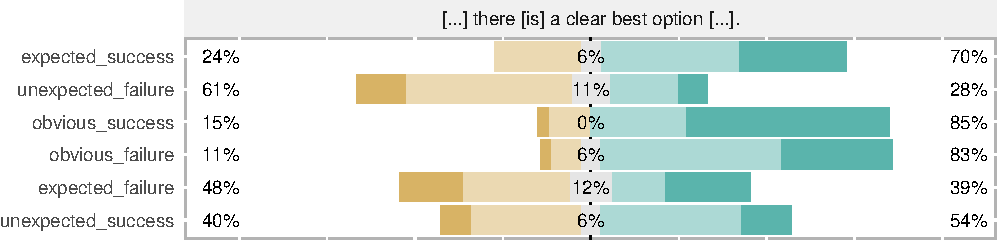
\includegraphics[width=\textwidth]{{fig/cropped-outcomes-report-01-opt.obvious}.pdf}
  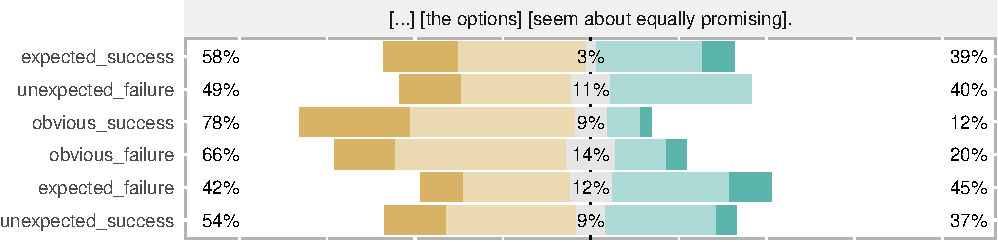
\includegraphics[width=\textwidth]{{fig/cropped-outcomes-report-02-opt.balanced}.pdf}
  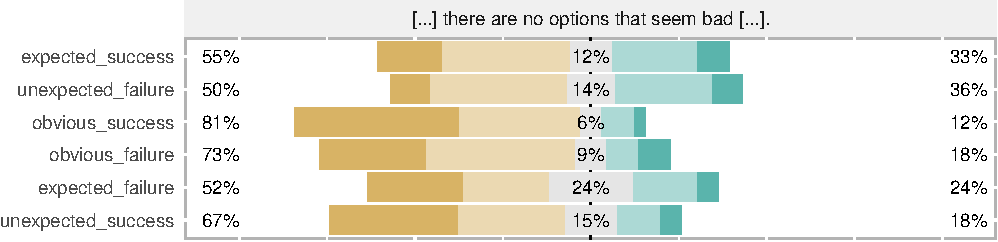
\includegraphics[width=\textwidth]{{fig/cropped-outcomes-report-03-opt.nobad}.pdf}
  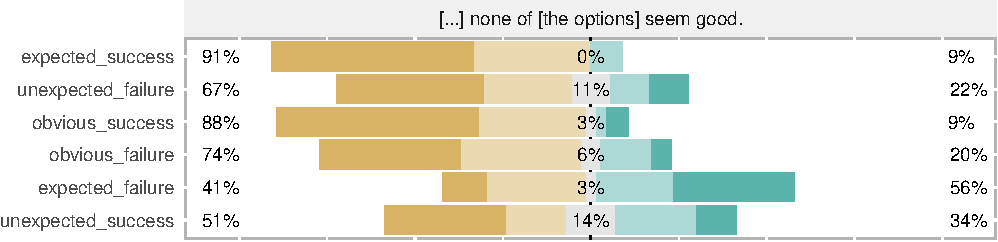
\includegraphics[width=\textwidth]{{fig/cropped-outcomes-report-04-opt.nogood}.pdf}
  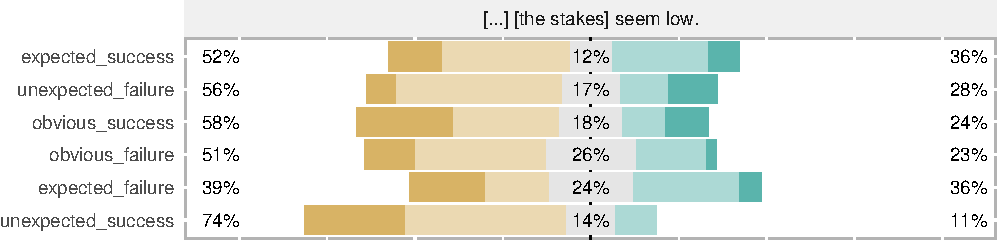
\includegraphics[width=\textwidth]{{fig/cropped-outcomes-report-05-opt.stakes}.pdf}
  
\includegraphics[width=\textwidth]{fig/outcomes-legend-custom.pdf}
  \caption[Retrospecitve option results]{Option-related results from the retrospective study. Cf. \cref{fig:e1-report}.}
  \label{fig:e2-option-report}
\end{figure}

\begin{figure}[!p]
  \centering
  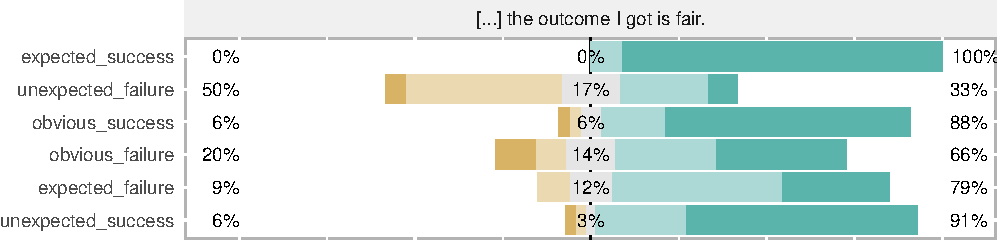
\includegraphics[width=\textwidth]{{fig/cropped-outcomes-report-10-out.fair}.pdf}
  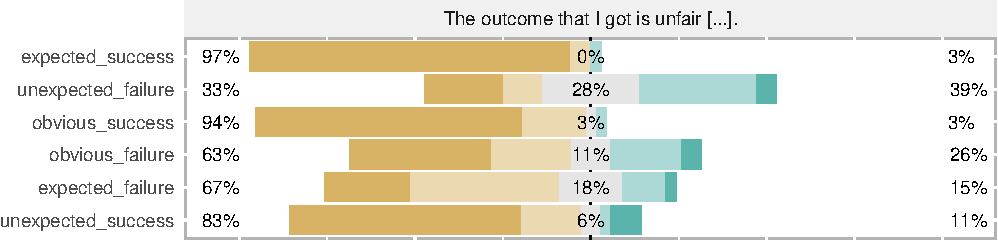
\includegraphics[width=\textwidth]{{fig/cropped-outcomes-report-11-out.unfair}.pdf}
  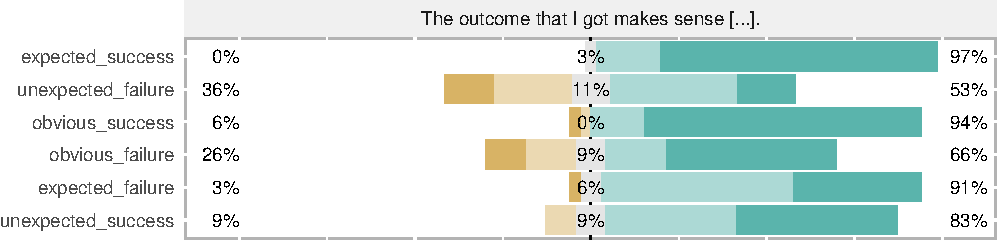
\includegraphics[width=\textwidth]{{fig/cropped-outcomes-report-12-out.sense}.pdf}
  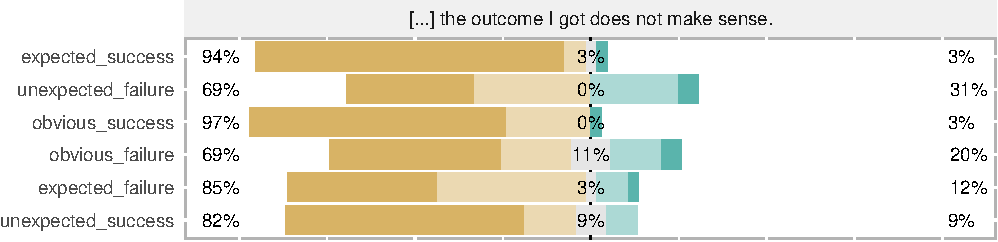
\includegraphics[width=\textwidth]{{fig/cropped-outcomes-report-13-out.broken}.pdf}
  
\includegraphics[width=\textwidth]{fig/outcomes-legend-custom.pdf}
  \caption[Retrospective fair/unfair \& sense/nonsense results]{Fair/unfair and sense/nonsense results from the retrospective study. Setup is the same as \cref{fig:e1-report}.}
  \label{fig:e2-outcome-report-fair-sense}
\end{figure}

\begin{figure}[!p]
  \centering
  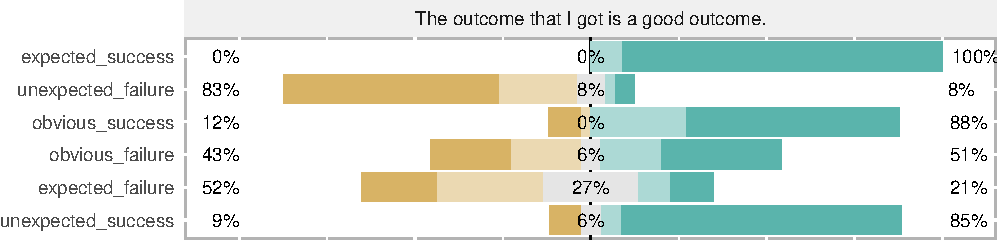
\includegraphics[width=\textwidth]{{fig/cropped-outcomes-report-06-out.good}.pdf}
  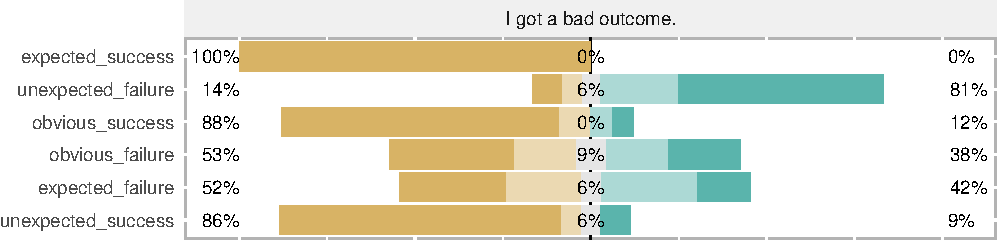
\includegraphics[width=\textwidth]{{fig/cropped-outcomes-report-07-out.bad}.pdf}
  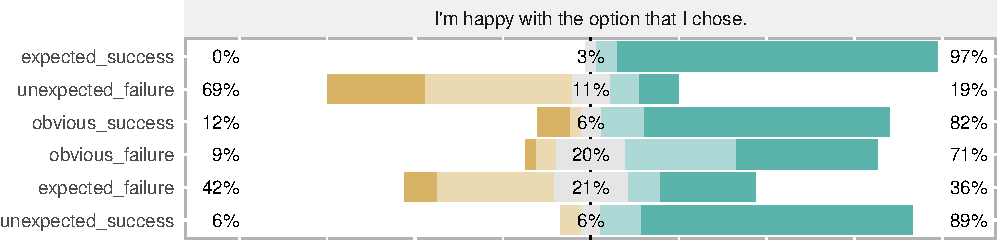
\includegraphics[width=\textwidth]{{fig/cropped-outcomes-report-14-out.happy}.pdf}
  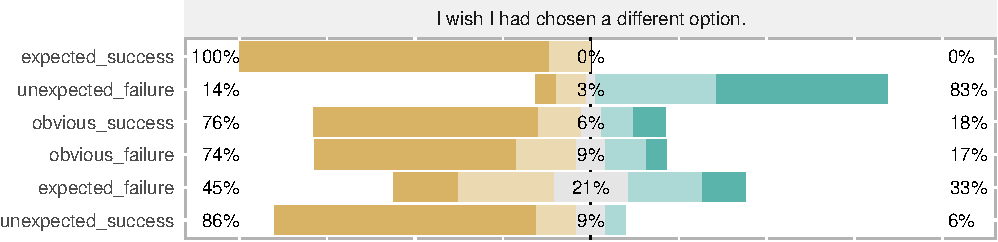
\includegraphics[width=\textwidth]{{fig/cropped-outcomes-report-15-out.regret}.pdf}
  
\includegraphics[width=\textwidth]{fig/outcomes-legend-custom.pdf}
  \caption[Retrospective good/bad \& satisifed/dissatisfied results]{Good/bad and satisfied/dissatisfied results from the retrospective study. Setup is the same as \cref{fig:e1-report}.}
  \label{fig:e2-outcome-report-valence-satisfaction}
\end{figure}

\begin{figure}[!t]
  \centering
  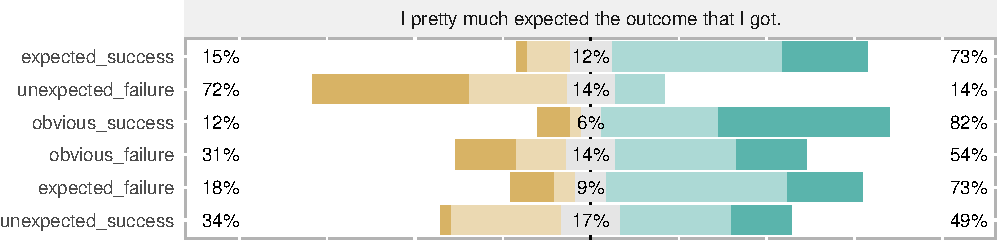
\includegraphics[width=\textwidth]{{fig/cropped-outcomes-report-08-out.expected}.pdf}
  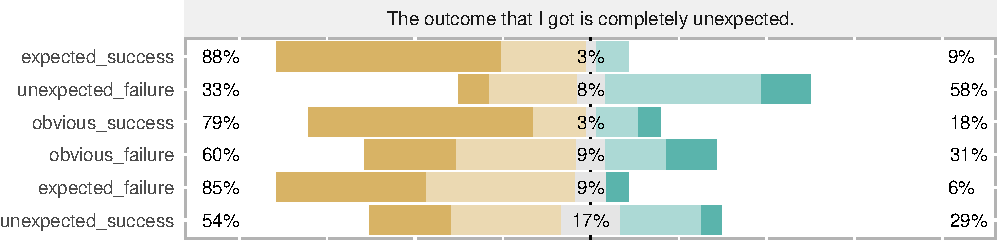
\includegraphics[width=\textwidth]{{fig/cropped-outcomes-report-09-out.unexpected}.pdf}
  
\includegraphics[width=\textwidth]{fig/outcomes-legend-custom.pdf}
  \caption[Retrospective expected/unexpected results]{Expected/unexpected retrospective results. Setup as in \cref{fig:e1-report}.}
  \label{fig:e2-outcome-report-surprise}
\end{figure}

\subsection{Summary}

A summary of the results appears in \cref{fig:e2-option-report,fig:e2-outcome-report-fair-sense,fig:e2-outcome-report-valence-satisfaction,fig:e2-outcome-report-surprise}, which have the same format as \cref{fig:e1-report}.
%
\Cref{fig:e2-option-report} includes all of the option-related questions, and can be compared directly to results in \cref{fig:e1-report}, especially for the last four conditions, which correspond in pairs to the \obv{} and \dlm{} conditions of the first experiment, respectively.
%
In \cref{fig:e2-outcome-report-fair-sense,fig:e2-outcome-report-valence-satisfaction,fig:e2-outcome-report-surprise}, the questions are ordered such that complimentary question pairs are adjacent, and comparing the data visually there seems to be a good deal of symmetry between these pairs, as expected.
%
Overall, the data indicate that \dunyazad/ is better at creating positive expectations and results than negative ones: compare the incredibly one-sided results for the \exps{} condition to the much more mixed results for \expf{,} for example.


As mentioned above, each of the rows in these figures represents between 32 and 36 responses, depending on the condition.
%
The sub-cases (e.g., \obvfm{} vs\@. \obvfa{}) are not separated here, although they are analyzed separately for some of the hypotheses.
%
For the \obvs{} condition, 25 of the 33 responses fell into the [main] sub-case, while the remaining 8 participants chose an option other than the one that \dunyazad/ expected would be most promising.
%
For the \obvf{} condition, the \casem{} sub-case contained 20 of the 35 responses, while the [alt] sub-case contained the remaining 15.
%
Note that each condition can be broken down into three individual choices, and there is a general expectation that these three choices will elicit generally similar responses, as they are constructed using the same set of constraints (although they are required to use three different setups).
%
Slight variation between choices within a condition should not disrupt the overall results, of course, but if there is significant divergence, it may be a sign that \dunyazad/'s internal reasoning about a choice doesn't agree with how participants experience that choice.


\section{Option Results}

\Cref{tab:e2-option-results} shows the results for the option-related hypotheses, with significant results listed in bold.
%
Note that in line with the results of the first study, none of the low-confidence hypotheses were supported by the data.
%
These hypotheses (marked with `\lc/') involved predictions which don't hold up if participants judge options relative to each other instead of in absolute terms, and the prospective study indicated strongly that this was the case for many participants.

\begin{table}[!t]
\centering
\bgroup
\def\arraystretch{1.3}
\setlength{\tabcolsep}{0.35em}
\begin{tabular}{r  c  c c c  c  c c c  c  c c c}
\toprule
\multirow{2}{5em}{\centering Question} &%
 & \multicolumn{3}{c}{\eIIexpectedsuccessabbr/} &%
 & \multicolumn{3}{c}{\eIIobvioussuccessabbr/} &%
 & \multicolumn{3}{c}{\eIIexpectedfailureabbr/} \\
&%
 & \multicolumn{3}{c}{\eIIunexpectedfailureabbr/} &%
 & \multicolumn{3}{c}{\eIIobviousfailureabbr/} &%
 & \multicolumn{3}{c}{\eIIunexpectedsuccessabbr/} \\
\midrule
\multirow{2}{5em}{\raggedleft \eIIoptobviousabbr/} &%
 & \tensig{D\lc/}{0.987} &%
 & \tesig{A}{$\bm{8.3\sqtimes 10^{-5}}$}{75\%} &%
 & \tensig{D\lc/}{0.467} \\
&%
 & \tensig{D\lc/}{0.128} &%
 & \tesig{A}{0.001}{70\%} &%
 & \tensig{D\lc/}{0.717} \\
\midrule
\multirow{2}{5em}{\raggedleft \eIIoptbalancedabbr/} &%
 & \tensig{A\lc/}{0.809} &%
 & \tesig{D}{0.003}{69\%} &%
 & \tensig{A\lc/}{0.485} \\
&%
 & \tensig{A\lc/}{0.767} &%
 & \tesig{D}{0.045}{61\%} &%
 & \tensig{A\lc/}{0.794} \\
\midrule
\multirow{2}{5em}{\raggedleft \eIIoptnobadabbr/} &%
 & \tensig{A\lc/}{0.807} &%
 & \tesig{D}{$\bm{4.5\sqtimes 10^{-4}}$}{72\%} &%
 & \tensig{D}{0.082} \\
&%
 & \tensig{A\lc/}{0.683} &%
 & \tesig{D}{0.013}{65\%} &%
 & \tesig{D}{0.011}{66\%} \\
\midrule
\multirow{2}{5em}{\raggedleft \eIIoptnogoodabbr/} &%
 & \tesig{D}{$\bm{1.1\sqtimes 10^{-5}}$}{78\%} &%
 & \tesig{D}{$\bm{4.1\sqtimes 10^{-5}}$}{76\%} &%
 & \tensig{A}{0.140} \\
&%
 & \tesig{D}{0.013}{65\%} &%
 & \tesig{D}{0.004}{68\%} &%
 & \tensig{A}{0.883} \\
\midrule
\multirow{2}{5em}{\raggedleft \eIIoptstakesabbr/} &%
 & \tensig{D}{0.279} &%
 & \tensig{D}{0.081} &%
 & \tensig{D}{0.310} \\
&%
 & \tensig{D}{0.257} &%
 & \tensig{D}{0.121} &%
 & \tesig{D}{0.003}{68\%} \\
\bottomrule
\end{tabular}

\egroup
\caption[Retrospective option results]{Option-related results in the retrospective experiment. Each row lists results for a single question; each column stacks results for two conditions (listed at the top) with identical \prq{option\_feel}{} constraints. Each entry indicates the hypothesis (`D' for `disagree' and `A' for `agree'), the $p$-value, and the common-language effect size for confirmed hypotheses (which are marked in bold instead of \nsighcolor/ where $p < 0.05$).} % TODO: Make this a one-liner to fit on the same page as the figure above...
  \label{tab:e2-option-results}
\end{table}


\subsection{Stakes}
One immediate pattern in these results is the lack of support for the ``low stakes'' hypotheses.
%
In our initial study, the hypothesis that choices which \dunyazad/ labelled as high-stakes would appear that way to participants was clearly confirmed by the data, with a $p$-value of 0.0011 and an effect size of 70\% (a strong effect).
%
In this study, every single choice was required to be high-stakes, but only in a single case (the \unxs{} condition) was the relevant hypothesis confirmed.
%
One reason why this might be the case is that in this study, \dunyazad/ was not allowed to control either the setup or the stakes of the choices, whereas in the initial study \dunyazad/ was free to control both.
%
The high-stakes choices in this study therefore necessarily included choices with \prq{market}{} setups, where it is impossible for \dunyazad/ to construct a scenario that directly threatens the player's character.
%
A breakdown of responses to the stakes question across all conditions by setup (\cref{fig:e2-stakes-by-setup}) seems to confirm that the \prq{market}{} setup is a problem: it elicits an even split between agree and disagree responses while the other two setups lean towards disagreeing.

To test this theory, I did a followup analysis with three hypotheses---each individual setup as a condition was hypothesized to elicit disagreement with the low stakes statement.
%
The results of this analysis confirmed my suspicions.
%
The test for the \prq{market}{} hypothesis does not reject the null hypothesis ($p = 0.502$), while the tests for the \prq{threatened\_innocents}{} and \prq{monster\_attack}{} hypotheses are confirmed ($p = 0.041$; effect size 60\% and $p = 0.0093$; effect size 64\% respectively).
%
Essentially, when \dunyazad/ creates choices without constraints regarding their stakes, the high-stakes choices that it does create are in fact perceived to be high-stakes by players.
%
However, when \dunyazad/ is specifically asked to create high-stakes choices using certain fixed setups, such as the \prq{market}{} setup, it doesn't manage to create choices that are convincingly high-stakes.
%
Whether this means that the perception of stakes has more to do with the setup text than the actual content of the options and/or outcomes is an open question that could be tested.

\begin{figure}[!t]
  \centering
  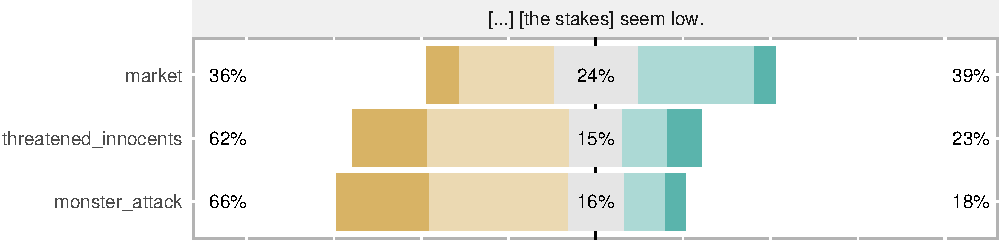
\includegraphics[width=\textwidth]{{fig/cropped-extra-outcomes-report-by-setup-05-opt.stakes}.pdf}
\hspace*{1.5pt}
\includegraphics[width=\textwidth]{fig/outcomes-legend-custom.pdf}
  \caption[Retrospective stakes results by setup]{Stakes results across all conditions grouped by the setup used.}
  \label{fig:e2-stakes-by-setup}
\end{figure}


\subsection{Expected Failure---No Bad Options?}

Besides the unconfirmed stakes hypotheses, there were two other places where high-confidence option-related hypothesis were not confirmed by the data.
%
The first is in the \expf{} case for the ``no bad'' statement.
%
Although the \unxs{} condition, which in theory generates options which set identical expectations, was confirmed to disagree with this statement, the data did not support this hypothesis for the \expf{} condition.
%
Of course, this condition is one susceptible to being undermined by relative value judgements: if all of the options seem bad, one might reason that it doesn't matter which is chosen, and therefore none of them are ``bad'' in the sense that choosing them would be a mistake.
%
It is telling that the \prq{obvious\_}{} cases confirmed corresponding hypotheses: when a single positive option was present alongside negative options, participants strongly rejected the notion that there were ``no bad options'' present.

\begin{figure}[!b]
  \centering
  {\sffamily Expected Failure}
  \includegraphics[width=\textwidth]{{fig/cropped-detailed-report-expected\string_failure-02-opt.nobad}.pdf}\\[1ex]
  {\sffamily Unexpected Success}
  \includegraphics[width=\textwidth]{{fig/cropped-detailed-report-unexpected\string_success-02-opt.nobad}.pdf}\\
  
\includegraphics[width=\textwidth]{fig/detailed-outcomes-legend-custom.pdf}
  \caption[Retrospective dilemma ``no bad options'' results]{Results for the ``no bad options'' statement in the \expf{} (top) and \unxs{} (bottom) conditions, grouped by choice. Each choice is identified by the numeric seed that was used to create it. The bracketed numbers on the right indicate the sample size for each choice.}
  \label{fig:e2-extra-nobad}
\end{figure}


But what about the difference between the \expf{} case and the \unxs{} case?
%
\Cref{fig:e2-extra-nobad} shows the results for each individual choice in both cases, and there isn't a clear culprit.
%
The choice with seed 58403 is the single choice among the six in that figure that elicited the most agreement with the statement, but it still tilts towards disagreement.
%
Given that both conditions include a substantial minority of ``agree'' and even ``strongly agree'' responses, there doesn't seem to be a clear underlying reason for the division in the results.
%
What is clear is that giving \dunyazad/ the ability to make relative rather than purely absolute value judgements should be a high priority.
%
In future studies, it might also be more productive to just ask participants to label each option as good/bad (and also suggests-success/suggests-failure), although as mentioned in the discussion of the setup for the first study, this kind of language promotes an analytical approach and that isn't necessarily desirable.


\begin{figure}[!b]
  \centering
  {\sffamily Expected Failure}
  \includegraphics[width=\textwidth]{{fig/cropped-detailed-report-expected\string_failure-03-opt.nogood}.pdf} \\[1ex]
  {\sffamily Unexpected Success}
  \includegraphics[width=\textwidth]{{fig/cropped-detailed-report-unexpected\string_success-03-opt.nogood}.pdf} \\
  
\includegraphics[width=\textwidth]{fig/detailed-outcomes-legend-custom.pdf}
  \caption[Retrospective dilemma ``no good options'' results]{Results for the ``no good options'' statement in the \expf{} (top) and \unxs{} (bottom) conditions, grouped by choice. The bracketed numbers in on the right indicate the sample size for each choice.}
  \label{fig:e2-extra-nogood}
\end{figure}


\subsection{Dilemma Cases---Competing Goals}

Another point of interest among the option-related results was the data's failure to support the hypotheses that the \expf{} and \unxs{} cases would be viewed as having ``no good options.''
%
Again, the \dlm{} case in the first experiment produced reactions that supported an equivalent hypothesis, so this result is somewhat surprising.
%
Here however the reasons for this discrepancy are clear.


\Cref{fig:e2-extra-nogood} shows the responses for these cases, and it is clear that the choices with seeds 87991, 8015, 47794, and 33152 are not yielding the expected results: participants are indicating that there is at least one good option at these choices.
%
\Cref{fig:e2-seed-87991} shows the choice with seed 87991, and the problem is immediately apparent: \dunyazad/ has used a \prq{travel\_onwards}{} action as a ``clearly bad result.''
%
This is a result of an overcorrection from the problems with \prq{travel\_onwards}{} that were discovered during the first study.
%
In that study, \prq{travel\_onwards}{} was a cure-all option which could get rid of any problem due to the way that it handled switching scenes.
%
For this second study, that bug was fixed, and instead, \prq{travel\_onwards}{} is marked as failing any goals relating to unresolved situations that it leaves behind. 
%
In this case, \dunyazad/ thinks that the  player will have an \prq{avoid\_accusations}{} goal with respect to the accused merchant, and simply leaving the merchant behind clearly fails this goal.

\begin{figure}[t]
\fseed{87991}
\caption[``Expected failure'' choice 87991]{The choice with seed 87991 minus the framing (which is mostly the same between choices). Boxed numbers before each outcome indicate the number of participants that chose that outcome. Note the popularity of the third option.}
\label{fig:e2-seed-87991}
\end{figure}


Of course, the underlying problem here is goal prioritization.
%
If given an good option to save the merchant, many players are eager to do so, but when such options are risky, they prefer to preserve their own safety.
%
With \dunyazad/'s two-level goal priority system, which was unchanged from the first experiment, it's not possible to represent this complexity.
%
Under the current system then, instead of \prq{travel\_onwards}{} being seen as an option with too few consequences, it is seen as an option with too many consequences.
%
The choice with seed 8015 also includes a \prq{travel\_onwards}{} option in a similar situation, and the inclusion of these options was likely the reason that players felt that the \expf{} cases actually \emph{did} have some good options.


\begin{figure}[h]
\fseed{47794}
\caption[``Unexpected success'' choice 47794]{The \unxs{} choice with seed 47794 minus its framing. Boxed numbers indicate the number of participants that selected each outcome.}
\label{fig:e2-seed-47794}
\end{figure}


\subsection{Dilemma Cases---Outcomes Affect Option Perception}

Recall that the \unxs{} case exhibited the same problem.
%
The reason for this was different, however, because neither the choice with seed 47794 nor the choice with seed 33152 had \prq{travel\_onwards}{} options.
%
Instead, the reason that these choices were rated as having at least one good option is probably their outcomes.
%
Because participants saw an outcome before answering any questions, the responses to the option questions could have been affected by the outcomes seen.
%
\Cref{fig:e2-seed-47794} shows the choice with seed 47794, and looking at it reveals a likely explanation for the ``no good options'' response.


As shown in that figure, six of ten participants who saw that choice chose the first option, and were ``unexpectedly'' successful.
%
But remember that \dunyazad/'s notion of what is expected is written in terms of system-wide rules: ``normally'' someone missing the negotiation skill should \emph{always} fail to talk someone else down, so if such an action succeeds the result is unexpected.
%
This kind of expectation is something that players would learn if they interacted with the system over a period of time, but participants in this study only saw a single choice.
%
Faced with a positive outcome, it would be natural to conclude that perhaps the negotiation skill isn't important after all, and therefore that the option that was chosen was a good one.
%
This line of reasoning would not be available to players before seeing an outcome, but as stated before, the risk of such influences was intentionally accepted as the price of a more natural decision-making experience.


Because the choice with seed 33152 included a very similar \prq{talk\_down}{} option which was also quite popular, this outcome-dependent effect can explain the failed hypothesis in the \unxs{} condition.
%
Unfortunately, the impact of this effect and the \prq{travel\_onwards}{} issue affecting the choices with seeds 87991 and 8015 is not negligible.
%
When it comes to evaluating the outcome-related hypotheses, these choices didn't convey the intended prospective poetics, and this could impact their retrospective poetics as well.


\subsection{Problems with \prq{travel\_onwards}{}}


Besides choices in the two dilemma conditions, two other choices---the \obvs{} choices with seeds 47371 and 20739---also included \prq{travel\_onwards}{} options.
%
These are shown in \cref{fig:e2-seeds-47371-20739}.
%
Luckily, the choice with seed 47371 happens to give participants an option that's more attractive than the \prq{travel\_onwards}{} option, so the same problem doesn't occur.
%
In fact, this is a good example of correct use of \prq{travel\_onwards}{} as an option that seems bad, which is reinforced by the fact that zero participants chose it.
%
However, based on the option popularities in choice 20739, that choice has the same problems as choices 87991 and 8015: the ``correct'' option involves some perceived risk or cost (in this case giving away an item to resolve the situation) and so simply ignoring the merchant's plight is seen as acceptable.


\begin{figure}[p]
\fseed{47371} \\
\fseed{20739}
\caption[``Obvious success'' choices 47371 and 20739]{The \obvs{} choices 47371 and 20739 minus framing. Boxed numbers indicate the number of participants who saw each outcome.}
\label{fig:e2-seeds-47371-20739}
\end{figure}


Note that these options are in the \obvs{} condition, and as such participants who saw them are divided into the \prq{[main]}{} and \prq{[alt]}{} sub-cases according to which option they chose.
%
For choice 47371, all 11 participants who chose option two are in the \prq{[main]}{} sub-case, while the other two participants are in the \prq{[alt]}{} sub-case.
%
For choice 20739, there are only two participants that the system thinks chose the ``correct'' option, and the majority of participants are put into the \prq{[alt]}{} sub-case.
%
This means that the meaning of the sub-cases is somewhat changed from its intent.
%
The \prq{[alt]}{} cases are supposed to consist of participants who intentionally chose a non-positive option despite the presence of a positive one, and as such they are assumed to be quite small, to the point that not many hypotheses were proposed which included \prq{[alt]}{} cases.
%
Because of \dunyazad/'s failure to predict the complexities of player goals, the \prq{[alt]}{} case consists largely of participants who thought they were choosing the best option available, but who disagreed with \dunyazad/'s evaluation of what that was.
%
Of course, although these effects diminish the number of participants in the \prq{[main]}{} cases, at least their meaning is not diluted very much: only a few participants from poorly-formed choices like 20739 wound up choosing the options that \dunyazad/ considered best, and so only a few participants in the \prq{[main]}{} cases weren't choosing what they thought was an obviously superior option.


\subsection{Costly Actions}

One failure in \dunyazad/'s reasoning here besides the inability to properly track goal priorities is it's focus on goals to the detriment of costs.
%
In other words, \dunyazad/ thinks about actions only in terms of the goals that they might achieve or threaten, and not in terms of the costs of those actions.
%
If the player must use an item to get what they want, \dunyazad/ neglects this cost and just sees that a goal is achieved.
%
Of course, this could be handled by adding player goals concerned with preserving resources, but the two-priority goal system doesn't leave room for such goals to affect high-stakes decisions even a little bit.

\begin{figure}[!b]
\fseed{95923}
\caption[``Obvious failure'' choice 95923]{The \obvf{} choice with seed 95923 minus framing. Boxed numbers indicate the number of participants that selected each outcome.}
\label{fig:e2-seed-95923}
\end{figure}


The choice with seed 20739 in \cref{fig:e2-seeds-47371-20739} is an example of this: In making a decision, even players who recognize that the first option will help the merchant have to somehow justify giving up their gold (and to a noble who doesn't deserve it, no less).
%
As the numbers indicate, most decided to simply travel onwards: the goal of helping the merchant was not worth the cost associated with it.
%
Of course, it doesn't help that the option text doesn't clearly state your intent in performing the action (to exonerate the merchant).\footnote{This issue has already been addressed by making the text more explicit for \prq{pay\_off}{} actions.}
%
In fact, one of the comments in the ``other'' free text response to the motivation question reveals exactly this kind of cost analysis in action:

\begin{quote}
  \quoteshape
You only really had 2 options. I wouldn't want to give up the gold if I didn't have to. So just negotiation made the most sense.
\end{quote}

This response was given by a participant who saw choice 95923, an \obvf{} choice shown in \cref{fig:e2-seed-95923}.
%
The fact that players are factoring costs into their decisions but \dunyazad/ is not tracking them is a problem.
%
Of course, the quote above reveals another problem: the choice with seed 95923 was supposed to be ``obvious'' choice with a single best option.
%
How did \dunyazad/ justify having two options that include positive skill indications?
%
In this case, \dunyazad/ has found what amounts to a loophole in its rules: the ``bad'' options at an obvious choice are allowed to be merely ``risky''---the reasoning is that compared to a really good option, a risky option will still be clearly inferior.
%
Because the \prq{talk\_down}{} action includes a risk that the target will begin accusing the initiator instead of their original victim, and because internally, having the negotiation skill doesn't guarantee success, \dunyazad/ views the first option as a ``risky'' one: one that has an unsubstantiated benefit but also a potential drawback.
%
Three factors combined to throw off \dunyazad/'s analysis.
%
First, the unaccounted-for cost of the ``good'' option meant that it really wasn't as attractive as it should have been.
%
Second, the fact that talking the noble down carried a risk wasn't something that was made clear from the surface text.
%
Third, the fact that in the first option, \dunyazad/ does not count the negotiation skill as decisive while in the second option it does creates a false equivalence at the surface text level: both options appear equally supported by the ``negotiation'' skill.


This problem of costliness was specific to the \prq{pay\_off}{} action, which was present in the five choices with seeds 20739, 95923, 40550, 67832, and 82994.
%
Choice 20739 was just discussed in the context of the \prq{travel\_onwards}{} action and choice 95923 is the choice that prompted this analysis, but the other three choices have not yet been considered.
%
Luckily, choice 40550 was a \unxf{} choice and choices 67832 and 82994 were both \exps{} choices: all three were in conditions that were supposed to have three good options.
%
As a result, these costly options were presented along with two actually-good options, and in fact the costly options at these choices were chosen by one, zero, and zero participants respectively.
%
In other words, these options probably had little effect on the outcome-related results, as they were almost never chosen.
%
On the other hand, they do compromise the \emph{option} structures of the choices in question, and so they have a potentially important effect on the between-cases comparisons.


One good thing in all of this is that none of the that \dunyazad/ is currently neglecting factors are fundamentally difficult to account for.
%
For example, the fact that all 12 participants at choice 95923 chose the first option, which can be deduced to be the best using some simple extensions to \dunyazad/'s current logic, means that \dunyazad/'s general strategy of using \emph{character} motivations to predict \emph{player} actions is probably on the right track.
%
Extending \dunyazad/'s option evaluation code to reason about action costs, handle complex goal priorities, and reason about directly-presented implications rather than implications implied by hidden action logic may be technically challenging, but it's a clear set of features to implement.
%
Despite \dunyazad/'s failures, the results of this study strongly imply that with these features, \dunyazad/ will be able to correctly predict player's option evaluations most of the time.


\section{Outcome Results}

While the results of the option-related hypotheses were somewhat lackluster, this was to some degree expected based on the results of the first study.
%
Had more improvements been made to \dunyazad/ before the second study, this might have been avoided, but the primary purpose of this study was to evaluate \dunyazad/'s outcome predictions, which had not been tested by the first study.
%
\Cref{tab:e2-positive-outcome-results,tab:e2-negative-outcome-results} show the results for nominally-positive- and nominally-negative-outcome conditions respectively (the top and bottom halves of \cref{tab:e2-outcome-hypotheses}).
%
Overall, \dunyazad/ seems to be generally successful at producing positive outcomes, although it has some trouble making them surprising.
%
On the other hand, its track-record for negative outcomes is not as good.
%
In particular, surprising negative outcomes were more consistently rated as actually being ``bad,'' but participants didn't necessarily accept the idea that they were ``unfair'' or ``nonsense.''

\begin{table}[!p]
\centering
\bgroup
\def\arraystretch{1.2}
\setlength{\tabcolsep}{0.4em}
\begin{tabular}{r  c@{\hspace{2em}}  c c c  c@{\hspace{2em}} c c c}
\toprule
\multirow{2}{5em}{\centering Question} &%
 & \multicolumn{3}{c}{\eIIexpectedsuccessabbr/} &%
 & \multicolumn{3}{c}{\eIIunexpectedsuccessabbr/} \\
&%
 & \multicolumn{3}{c}{\eIIobvioussuccessmainabbr/} &%
 & \multicolumn{3}{c}{\eIIobviousfailurealtabbr/} \\
\midrule
\multirow{2}{6em}{\raggedleft \hangpara{1.3em}{1}\eIIoutfairabbr/} &%
 & \tesig{A}{$\bm{6.8\sqtimes 10^{-11}}$}{88\%} &%
 & \tesig{A}{$\bm{1.6\sqtimes 10^{-6}}$}{80\%} \\
&%
 & \tesig{A}{$\bm{1.7\sqtimes 10^{-8}}$}{87\%} &%
 & \tesig{A}{$\bm{1.1\sqtimes 10^{-5}}$}{85\%} \\
\midrule
\multirow{2}{6em}{\raggedleft \hangpara{1.3em}{1}\eIIoutunfairabbr/} &%
 & \tesig{D}{$\bm{2.7\sqtimes 10^{-10}}$}{87\%} &%
 & \tesig{D}{$\bm{3.5\sqtimes 10^{-5}}$}{76\%} \\
&%
 & \tesig{D}{$\bm{1.7\sqtimes 10^{-8}}$}{87\%} &%
 & \tesig{D}{$\bm{4.2\sqtimes 10^{-6}}$}{86\%} \\
\midrule
\multirow{2}{6em}{\raggedleft \hangpara{1.3em}{1}\eIIoutsenseabbr/} &%
 & \tesig{A}{$\bm{8.2\sqtimes 10^{-9}}$}{85\%} &%
 & \tesig{A}{$\bm{1.3\sqtimes 10^{-4}}$}{74\%} \\
&%
 & \tesig{A}{$\bm{4.7\sqtimes 10^{-8}}$}{85\%} &%
 & \tesig{A}{$\bm{4.2\sqtimes 10^{-6}}$}{86\%} \\
\midrule
\multirow{2}{6em}{\raggedleft \hangpara{1.3em}{1}\eIIoutbrokenabbr/} &%
 & \tesig{D}{$\bm{6.9\sqtimes 10^{-9}}$}{85\%} &%
 & \tesig{D}{$\bm{7.1\sqtimes 10^{-6}}$}{78\%} \\
&%
 & \tesig{D}{$\bm{1.7\sqtimes 10^{-6}}$}{82\%} &%
 & \tesig{D}{$\bm{1.1\sqtimes 10^{-5}}$}{85\%} \\
\midrule
\multirow{2}{6em}{\raggedleft \hangpara{1.3em}{1}\eIIoutgoodabbr/} &%
 & \tesig{A}{$\bm{6.8\sqtimes 10^{-11}}$}{88\%} &%
 & \tesig{A}{$\bm{1.5\sqtimes 10^{-6}}$}{79\%} \\
&%
 & \tesig{A}{$\bm{3.4\sqtimes 10^{-7}}$}{84\%} &%
 & \tesig{A}{$\bm{4.2\sqtimes 10^{-6}}$}{86\%} \\
\midrule
\multirow{2}{6em}{\raggedleft \hangpara{1.3em}{1}\eIIoutbadabbr/} &%
 & \tesig{D}{$\bm{6.7\sqtimes 10^{-13}}$}{90\%} &%
 & \tesig{D}{$\bm{9.2\sqtimes 10^{-7}}$}{80\%} \\
&%
 & \tesig{D}{$\bm{1.3\sqtimes 10^{-7}}$}{84\%} &%
 & \tesig{D}{$\bm{4.2\sqtimes 10^{-6}}$}{86\%} \\
\midrule
\multirow{2}{6em}{\raggedleft \hangpara{1.3em}{1}\eIIouthappyabbr/} &%
 & \tesig{A}{$\bm{1.7\sqtimes 10^{-10}}$}{88\%} &%
 & \tesig{A}{$\bm{1.4\sqtimes 10^{-7}}$}{82\%} \\
&%
 & \tesig{A}{$\bm{4.7\sqtimes 10^{-8}}$}{85\%} &%
 & \tesig{A}{$\bm{1.5\sqtimes 10^{-6}}$}{87\%} \\
\midrule
\multirow{2}{6em}{\raggedleft \hangpara{1.3em}{1}\eIIoutregretabbr/} &%
 & \tesig{D}{$\bm{2.2\sqtimes 10^{-10}}$}{88\%} &%
 & \tesig{D}{$\bm{4.8\sqtimes 10^{-7}}$}{81\%} \\
&%
 & \tesig{D}{$\bm{1.1\sqtimes 10^{-6}}$}{82\%} &%
 & \tesig{D}{$\bm{1.5\sqtimes 10^{-6}}$}{87\%} \\
\midrule
\multirow{2}{6em}{\raggedleft \hangpara{1.3em}{1}\eIIoutexpectedabbr/} &%
 & \tesig{A}{0.011}{66\%} &%
 & \tensig{D}{0.795} \\
&%
 & \tesig{A}{$\bm{3.0\sqtimes 10^{-4}}$}{75\%} &%
 & \tensig{D}{0.996} \\
\midrule
\multirow{2}{6em}{\raggedleft \hangpara{1.3em}{1}\eIIoutunexpectedabbr/} &%
 & \tesig{D}{$\bm{6.6\sqtimes 10^{-6}}$}{78\%} &%
 & \tensig{A}{0.896} \\
&%
 & \tesig{D}{$\bm{3.0\sqtimes 10^{-4}}$}{75\%} &%
 & \tensig{A}{0.997} \\
\bottomrule
\end{tabular}

\egroup
\caption[Retrospective positive outcome results]{The results from the retrospective study for conditions that have nominally positive outcomes. Each row stacks results from the two (sub-)conditions listed at the top. Each result lists the hypothesis (`A' for agree or `D' for disagree), the p-value, and if significant ($p < 0.05$) the common-language effect size.}
  \label{tab:e2-positive-outcome-results}
\end{table}

\begin{table}[!p]
\centering
\bgroup
\def\arraystretch{1.2}
\setlength{\tabcolsep}{0.4em}
\begin{tabular}{l  c  c c c  c  c c c}
\toprule
\multirow{2}{5em}{Question} &%
 & \multicolumn{3}{c}{Expected Failure} &%
 & \multicolumn{3}{c}{Unexp. Failure} \\
&%
 & \multicolumn{3}{c}{Obv. Success [alt]} &%
 & \multicolumn{3}{c}{Obv. Failure [main]} \\
\toprule
\midrule
\multirow{2}{8em}{\hangpara{1.3em}{1}\sIIoutfairabbr/} &%
 & \tesig{A}{0.001}{68\%} &%
 & \tensig{D}{0.343} \\
&%
 & \tensig{A}{0.274} &%
 & \tensig{D}{0.460} \\
\midrule
\multirow{2}{8em}{\hangpara{1.3em}{1}\sIIoutunfairabbr/} &%
 & \tesig{D}{0.017}{63\%} &%
 & \tensig{A}{0.634} \\
&%
 & \tesig{D}{0.024}{65\%} &%
 & \tensig{A}{0.419} \\
\midrule
\multirow{2}{8em}{\hangpara{1.3em}{1}\sIIoutsenseabbr/} &%
 & \tesig{A}{$\bm{1.2\sqtimes 10^{-4}}$}{72\%} &%
 & \tensig{D}{0.716} \\
&%
 & \tesig{A}{0.012}{67\%} &%
 & \tensig{D}{0.508} \\
\midrule
\multirow{2}{8em}{\hangpara{1.3em}{1}\sIIoutbrokenabbr/} &%
 & \tesig{D}{$\bm{4.2\sqtimes 10^{-4}}$}{70\%} &%
 & \tensig{A}{0.981} \\
&%
 & \tesig{D}{$\bm{6.2\sqtimes 10^{-4}}$}{74\%} &%
 & \tensig{A}{0.783} \\
\midrule
\multirow{2}{8em}{\hangpara{1.3em}{1}\sIIoutgoodabbr/} &%
 & \tensig{D}{0.129} &%
 & \tesig{D}{$\bm{2.6\sqtimes 10^{-5}}$}{73\%} \\
&%
 & \tensig{D}{0.519} &%
 & \tesig{D}{0.006}{67\%} \\
\midrule
\multirow{2}{8em}{\hangpara{1.3em}{1}\sIIoutbadabbr/} &%
 & \tensig{A}{0.762} &%
 & \tesig{A}{$\bm{1.7\sqtimes 10^{-4}}$}{71\%} \\
&%
 & \tensig{A}{0.919} &%
 & \tesig{A}{0.014}{65\%} \\
\midrule
\multirow{2}{8em}{\hangpara{1.3em}{1}\sIIouthappyabbr/} &%
 & \tenp  &%
 & \tesig{D}{0.024}{62\%} \\
&%
 & \tenp  &%
 & \tensig{D}{0.809} \\
\midrule
\multirow{2}{8em}{\hangpara{1.3em}{1}\sIIoutregretabbr/} &%
 & \tenp  &%
 & \tesig{A}{$\bm{3.7\sqtimes 10^{-4}}$}{70\%} \\
&%
 & \tenp  &%
 & \tensig{A}{0.897} \\
\midrule
\multirow{2}{8em}{\hangpara{1.3em}{1}\sIIoutexpectedabbr/} &%
 & \tesig{A}{0.031}{61\%} &%
 & \tesig{D}{$\bm{9.5\sqtimes 10^{-4}}$}{68\%} \\
&%
 & \tensig{A}{0.129} &%
 & \tensig{D}{0.168} \\
\midrule
\multirow{2}{8em}{\hangpara{1.3em}{1}\sIIoutunexpectedabbr/} &%
 & \tesig{D}{$\bm{2.9\sqtimes 10^{-4}}$}{70\%} &%
 & \tensig{A}{0.184} \\
&%
 & \tesig{D}{0.036}{64\%} &%
 & \tensig{A}{0.313} \\
\bottomrule
\end{tabular}

\egroup
\caption[Retrospective negative outcome results]{The results from the retrospective study for conditions that have nominally negative outcomes. The format is the same as that of \cref{tab:e2-positive-outcome-results}.}
\label{tab:e2-negative-outcome-results}
\end{table}


\subsection{Outcomes and Option Perception (Again)}

The only hypotheses regarding nominally successful outcomes that weren't confirmed were those regarding the expectedness of the nominally unexpected cases.
%
These two conditions, the \unxs{} and \obvfa{} conditions, were supposed to be cases where a participant chose an option which carried some indicator that it would fail, but got a successful result.
%
The choices involved had seeds 99500, 47794, and 33152 (\unxs{}); and 8638, 28306, and 95923 (\obvf{}).
%
Of course, only participants who didn't choose the nominally best option at choices 8638, 28306, and 95923 fell into the \obvfa{} case.


Unfortunately, the failure to confirm these hypotheses is not terribly surprising: out of all of the outcome-related statements, the statements about expectedness and unexpectedness are the most heavily dependent on participant's perception of the option text as opposed to only the outcome text.
%
Because several of the choices listed above had problems with option perceptions, they didn't really fit the outcome profile that the hypotheses were expecting.
%
Choices 47794 (see \cref{fig:e2-seed-47794}) and 33152 (not shown) together account or 24 of the 35 \unxs{} responses, and as already discussed, they each included a popular option that \emph{in light of its outcome} did not seem like a bad option.
%
Because the option text along didn't give players a strong negative expectation for these options, positive results were not only not surprising; they made the option seem like it had been a good one from the start.


The fact that participants marked the outcomes of these options as expected might also point to a different effect: player trust in game-like systems.
%
In most modern games, unless the player has already received substantial warnings that they are on the wrong path, there won't be choices that have no ``correct'' option: even the worst situations will have some means of escape if the player is thrust into them without control over prior situations.
%
Because participants in this study only saw one choice, they may have assumed that there would be a ``correct'' option that would lead to a successful result.
%
With this expectation in mind, it's not surprising at all that choosing what one thinks is the best result will lead to a good outcome, even if the option text includes some negative indicator.


From the perspective of choice poetics, both of these possible effects are important to keep in mind.
%
First is the idea that options and outcomes both influence the perception of the other.
%
In this case, because \dunyazad/ did not make clearly bad-seeming options, a positive outcome was able to make those options seem like good options (at the very least, relative to other options at those choices).
%
Of course, given that those options seemed good, the notion that a good outcome would be surprising was no longer valid.
%
In other words, players reason neither strictly from options to outcomes nor from outcomes to options, but their perceptions of both affect their perceptions of the other.
%
If fact, there is ample evidence of this kind of reasoning even in real-world decisions (for an extreme example see studies on choice blindness such as \citep{Hall2012}).
%
If an author is interested in constructing an option that feels a specific way in retrospect, then, they must be mindful of the consequences of that option.


If the fact that options meant to seem indicative of failure were not explains the expectedness result in the \unxs{} case, what about the \obvfa{} case?
%
Choice 95923 from that case has already appeared here as well (see \cref{fig:e2-seed-95923}) and in combination with a graph of all responses to the ``expected'' question in \obvfa{} cases (\cref{fig:e2-obvious-failure-detail}) explains what is going on.
%
Essentially, \dunyazad/'s failure to make choice 95923 obvious flooded the \obvfa{} sub-case with 12 responses that dominated the three from the other two choices (which were clearly much better at getting participants to choose the intended choice).
%
The \obvfa{} sub-case therefore does not mainly consist of players who chose a bad option but got a good result.
%
Instead, it mainly consists of players who chose option one at choice 95923, which as already discussed, seemed to be a clearly positive option.
%
Because of this, getting a good result was not surprising, and the corresponding hypotheses were not confirmed.

\begin{figure}[!b]
  \centering
  {\sffamily Obvious Failure [alt]}
  \includegraphics[width=\textwidth]{{fig/cropped-detailed-report-obvious\string_failure(alt)-08-out.expected}.pdf}
  
\includegraphics[width=\textwidth]{fig/detailed-outcomes-legend-custom.pdf}
  \caption[Retrospective obvious failure ``expected'' results]{Results for the ``expected'' statement in the \obvfa{} sub-case, grouped by seed. Note the bracketed numbers on the right which indicate the sample size for each choice: seed 95923 dominates this category.}
  \label{fig:e2-obvious-failure-detail}
\end{figure}

\subsection{Outcome Text vs\@. States}

\begin{figure}[!p]
\centering%
\fseed{99500}\\[1ex]
{ \sffamily Unexpected Success}\\
\includegraphics[width=\textwidth]{{fig/cropped-detailed-report-unexpected\string_success-06-out.bad}.pdf}\\
\includegraphics[width=\textwidth]{{fig/cropped-detailed-report-unexpected\string_success-10-out.good}.pdf}\\

\includegraphics[width=\textwidth]{fig/detailed-outcomes-legend-custom.pdf}
\caption[``Unexpected success'' valence results and choice 99500]{The choice with seed 99500 along with valence results from the \unxs{} condition. Boxed values indicate the number of participants that selected each outcome at choice 99500, and bracketed numbers on the right of the graph below indicate sample sizes for each row. Note the diverging responses for choice 99500 and the text of the outcome for option one.}
\label{fig:e2-seed-99500-plus}
\end{figure}

Before moving on to discuss the nominally-negative outcome hypotheses, there's one more choice that didn't quite give expected results from the \unxs{} condition.
%
This is choice 99500 (shown in \cref{fig:e2-seed-99500-plus}), which stood out because a sizeable minority felt that the outcome they got was bad.
%
Inspecting the choice reveals the problem: the result of option one includes outcome text that seems at odds with itself: ``you are defeated,'' but the ogre is ``no longer threatening you'' and ``she is now injured.''
%
Within the system of outcome constraints placed on the \prq{attack}{} action, this is allowed: defeat of the target precludes the death of the attacker, but they may still be injured.
%
The real problem here is that the ``defeated'' outcome does not have any direct effects on the state of the world, unless the defeated party is threatening or accusing someone, in which case those states are removed.


Because \dunyazad/ generated a ``defeat'' with no negative consequences attached in terms of world state, it viewed that ``defeat'' as it would a victory: state changes effected by the action are unambiguously positive for the player, so the result is a ``success.''
%
Of course, participants felt otherwise: of the four participants that selected that option, three gave the anomalous responses to the valence questions shown in \cref{fig:e2-seed-99500-plus} and the fourth supplied both neutral responses.
%
The disconnect here between the text and \dunyazad/'s internal representation of the world causes a rift between its predictions and player's actual impressions.
%
In this case, the effect was isolated enough that it didn't upset any hypotheses, but forcing a clear link between every outcome reflected in the text and a definite internal state would help avoid situations like this.


\subsection{The Outcome of \prq{travel\_onwards}{}}

\begin{figure}[t]
  \centering
  {\sffamily Expected Failure}\\
\includegraphics[width=\textwidth]{{fig/cropped-detailed-report-expected\string_failure-06-out.bad}.pdf}\\
\includegraphics[width=\textwidth]{{fig/cropped-detailed-report-expected\string_failure-10-out.good}.pdf}\\[1ex]
{\sffamily Obvious Success [alt]}\\
\includegraphics[width=\textwidth]{{fig/cropped-detailed-report-obvious\string_success(alt)-06-out.bad}.pdf}\\
\includegraphics[width=\textwidth]{{fig/cropped-detailed-report-obvious\string_success(alt)-10-out.good}.pdf}\\
\hspace*{2pt}
\includegraphics[width=\textwidth]{fig/detailed-outcomes-legend-custom.pdf}
\caption[``Expected failure'' valence results]{Results for the ``good'' and ``bad'' items from the \expf{} and \obvsa{} conditions. Bracketed numbers on the right indicate sample sizes for each row; note that the \obvsa{} condition is dominated by choice 20739, and even then has only 8 samples in total.}
\label{fig:e2-expected-failure-detail}
\end{figure}

As already mentioned, in its present state \dunyazad/ views \prq{travel\_onwards}{} actions as much more negative than participants, who often found simply ignoring a problem to be an acceptable choice.
%
This was not only true of option perceptions, but of outcome perceptions as well.
%
In fact, the failure of \expf{} and \obvsa{} choices to give reliably negative results (shown in \cref{tab:e2-negative-outcome-results}) can be attributed to this problem.
%
As shown in \cref{fig:e2-expected-failure-detail}, which graphs responses to the ``good'' and ``bad'' statements for the \expf{} and \obvsa{} conditions, the choices where a majority of participants felt that the outcome was positive are all choices containing \prq{travel\_onwards}{} options (choices 87991, 8015, and 20739, discussed above).
%
These \prq{travel\_onwards}{} options, which the system considers to be unambiguously bad (because the player's character fails to help someone in need), are seen by players as a good or at least mixed result: they have successfully avoided an otherwise troublesome situation.
%
The presence of these options neatly explains the left-hand column of \cref{tab:e2-negative-outcome-results}: they aren't viewed as bad, but they are seen as fair, sensible, and expected.
%
The only remaining unconfirmed hypotheses are those for the \obvsa{} sub-case, but those can also be explained with reference to \cref{fig:e2-expected-failure-detail}: the simple lack of data for the \casea{} sub-case of the \obvs{} condition (eight responses total) makes such hypotheses difficult to confirm statistically.
%
The fact that the bulk of the \obvsa{} case responses (5) were from participants who selected to \prq{travel\_onwards}{} at choice 20739 (cf. \cref{fig:e2-seeds-47371-20739}) didn't help matters.

\begin{figure}[p]
  \centering
  {\sffamily Unexpected Failure}\\
\includegraphics[width=\textwidth]{{fig/cropped-detailed-report-unexpected\string_failure-09-out.fair}.pdf}\\
\includegraphics[width=\textwidth]{{fig/cropped-detailed-report-unexpected\string_failure-15-out.unfair}.pdf}\\
\includegraphics[width=\textwidth]{{fig/cropped-detailed-report-unexpected\string_failure-13-out.sense}.pdf}\\
\includegraphics[width=\textwidth]{{fig/cropped-detailed-report-unexpected\string_failure-07-out.broken}.pdf}
{\sffamily Obvious Failure [main]}\\
\includegraphics[width=\textwidth]{{fig/cropped-detailed-report-obvious\string_failure(main)-09-out.fair}.pdf}\\
\includegraphics[width=\textwidth]{{fig/cropped-detailed-report-obvious\string_failure(main)-15-out.unfair}.pdf}\\
\includegraphics[width=\textwidth]{{fig/cropped-detailed-report-obvious\string_failure(main)-13-out.sense}.pdf}\\
\includegraphics[width=\textwidth]{{fig/cropped-detailed-report-obvious\string_failure(main)-07-out.broken}.pdf}
\caption[Unexpected failure fairness and sense results]{Results for the fairness and sense items in the \unxf{} and \obvfm{} conditions. Bracketed numbers on the right indicate sample sizes for each row. Scale as per previous figures.}
\label{fig:e2-unexpected-failure-detail-fair-sense}
\end{figure}


\subsection{Fairness and The Strength of Expectations}

Examining the \emph{unexpected} failure conditions (the right half of \cref{tab:e2-negative-outcome-results}) it is immediately apparent that participants found them to be more fair and less broken than expected.
%
The relevant rows of \cref{fig:e2-outcome-report-fair-sense} indicate that these two conditions did stand out as the \emph{least} fair and \emph{most} broken cases, but they were not found to be more unfair than fair or more broken than sensible as expected.
%
\Cref{fig:e2-unexpected-failure-detail-fair-sense} breaks down the responses by individual choice, and gives a sense as to which choices were viewed as more fair (and/or less broken) than others.
%
In the \unxf{} condition, the choice with seed 46585 stands out as seeming more fair than its companions, and in the \obvfm{} condition, the choice with seed 28306 seems to be the culprit.


\begin{figure}[!b]
\fseed{46585}
\caption[``Unexpected failure'' choice 46585]{The \unxf{} choice with seed 46585. Boxed numbers indicate the number of participants who selected each outcome.}
\label{fig:e2-seed-46585}
\end{figure}


\Cref{fig:e2-seed-46585,fig:e2-seed-28306} display the choices in question, and they share a common property that's likely related to why they were seen as fair: despite their differing option structures, they include options which generate only weak expectations of success, and which have somewhat mixed results.
%
In choice 46585, both the first and third options involve some kind of debate, and while the ``negotiation'' skill probably helps debate successfully, it's not the kind of action where the result would ever be a forgone conclusion.
%
The same is true in choice 28306: the attack option involves fighting, which is an action often prone to unexpected results, and furthermore, the advantage ascribed to the player in the option text is only marginal: possession of a weapon when both parties have the relevant skill.

\begin{figure}[t]
\fseed{28306}
\caption[``Obvious failure'' choice 28306]{The \obvf{} choice with seed 28306. Boxed numbers indicate the number of participants who selected each outcome.}
\label{fig:e2-seed-28306}
\end{figure}


Besides the fact that these choices don't set up strong expectations with their option text, they also don't have unreservedly negative results.
%
For example, in the third outcome of choice 46585, while it's true that failing to get rid of an accusation as intended is a bad thing, it's not necessarily awful: maybe the player will get another chance to address the situation before something really bad happens.
%
Similarly in outcome three of choice 28306, despite sustaining an injury the overall battle ends in a draw.
%
While these \emph{are} negative outcomes (and the results show that participants understood this), are they negative enough to be considered ``unfair'' with respect to the expectations set up by the option text?
%
The subjects in our study didn't think so, and thus our hypotheses that these conditions would be perceived as unfair and possibly broken were not supported.

\begin{figure}[!t]
\fseed{8638}
\caption[``Obvious failure'' choice 8638]{The \obvf{} choice with seed 8638. Boxed numbers indicate the number of participants who selected each outcome. This is an example of \dunyazad/ successfully creating a choice that participants viewed as unfair.}
\label{fig:e2-seed-8638}
\end{figure}


In \dunyazad/'s internal calculus, these options all simply ``suggest success,'' and ``result in failure'' but evaluating them in human terms shows that the expectations that they set up are limited.
%
The contrast between these options and ones which players overwhelmingly found to be unfair (such as option two of choice 8638, shown in \cref{fig:e2-seed-8638}) is illustrative.
%
Choice 8638 combines an obvious option structure (so players feel they are making the correct decision by picking option two) with a disappointing failure.
%
The desire to see the results of the polymorph spell might have something to do with the strong reactions to choice 8638, but the fact that the option text of option two mentions two positive factors and no negative ones is likely important as well.
%
If an author is intentionally trying to create a choice that is perceived as unfair, it seems that being subtle when suggesting a positive outcome is a dangerous approach.


\subsection{Regret and Alternatives}
\label{sec:results-about-regret}

Another unexpected result in the unexpected failure column was the fact that participants weren't dissatisfied with their decisions at \obvf{} choices.
%
In retrospect, these hypotheses were poorly thought out: the \obvfm{} case should one in which a participant selects what appears to be the only available good option, but is given a negative outcome.
%
Although one would expect such outcomes to be perceived as bad (which they were), the questions about satisfaction were asking whether participants \emph{would rather have picked a different option.}
%
If a participant truly thinks that the option they picked is the only good option, then despite a negative result, they should not believe that picking a different option would lead to a better outcome.
%
Of course, it's not the case that they clearly \emph{wouldn't} want to try a different option---the outcome they got \emph{was} bad---so neither enthusiastic agreement nor firm denial seem like appropriate responses.


The answers that we got reflected these competing impulses: the ``satisfied'' and ``dissatisfied'' statements both received a substantial number of neutral responses in the \obvfm{} condition, and the non-neutral responses were about evenly split overall, as shown in \cref{fig:e2-obvious-failure-main-detail-regret-expected}.
%
\Cref{fig:e2-seed-8638,fig:e2-seed-28306} (just shown) show the two choices that had any \casem{} responses in the \obvf{} condition; the data in \cref{fig:e2-obvious-failure-main-detail-regret-expected} all comes from the 20 participants who chose the most popular options at one of those choices.
%
While choice both choices are split, choice 28306 leans a bit more towards satisfaction, which may reflect being perceived as more fair, as just discussed.
%
Ultimately, the hypotheses that the \obvfm{} case would leave players feeling dissatisfied with their choice was shortsighted, and the mixed results that we got should have been expected given the tension between a bad result and a lack of viable alternatives produced by these choices.


\subsection{Expectations and... Expectedness}

\begin{figure}[!b]
  \centering
{\sffamily Obvious Failure [main]}\\
\includegraphics[width=\textwidth]{{fig/cropped-detailed-report-obvious\string_failure(main)-11-out.happy}.pdf}\\
\includegraphics[width=\textwidth]{{fig/cropped-detailed-report-obvious\string_failure(main)-12-out.regret}.pdf}\\
\includegraphics[width=\textwidth]{{fig/cropped-detailed-report-obvious\string_failure(main)-08-out.expected}.pdf}\\
\includegraphics[width=\textwidth]{{fig/cropped-detailed-report-obvious\string_failure(main)-14-out.unexpected}.pdf}\\

\includegraphics[width=\textwidth]{fig/detailed-outcomes-legend-custom.pdf}
\caption[Obvious failure (main) regret and expectedness results]{Results for the satisfaction and expectedness items in the \obvfm{} condition. Bracketed numbers on the right indicate sample sizes for each row.}
\label{fig:e2-obvious-failure-main-detail-regret-expected}
\end{figure}

The differences between choices 8638 and 28306 in terms of perceived fairness, brokenness, and satisfaction have been discussed, but there is one more pair of hypotheses relating to these choices that was not confirmed: the hypotheses stating that their results would be unexpected.
%
However, the issue of their differing expectations has already been discussed in relation to perceptions of fairness.
%
If choice 28306 is perceived as more fair because it gives rise to weaker expectations of success, then its negative result should be less unexpected than that of choice 8638.
%
Looking at the bottom two graphs in \cref{fig:e2-obvious-failure-main-detail-regret-expected}, this is exactly what was observed.


\begin{figure}[!b]
  \centering
{\sffamily Unexpected Failure}\\
\includegraphics[width=\textwidth]{{fig/cropped-detailed-report-unexpected\string_failure-08-out.expected}.pdf}\\
\includegraphics[width=\textwidth]{{fig/cropped-detailed-report-unexpected\string_failure-14-out.unexpected}.pdf}\\
\includegraphics[width=\textwidth]{fig/detailed-outcomes-legend-custom.pdf}
\caption[Unexpected failure expectedness results]{Results for the expectedness items in the \unxf{} condition. Bracketed numbers on the right indicate sample sizes for each row.}
\label{fig:e2-unexpected-failure-detail-unexpected}
\end{figure}


The weak positive expectations in choice 28306 are thus largely responsible for the failure of the \obvfm{} sub-case's results to be viewed as unexpected.
%
Of course, another factor was the makeup of choice 95923, the third \obvf{} choice, which did not contribute any samples to the \casem{} case.
%
If just choice 8638 is considered, the hypotheses that its outcome was unexpected are confirmed ($p=0.01337$, effect size 72\% for the ``not expected'' hypothesis and $p=0.014$, effect size 72\% for the ``was unexpected'' hypothesis) even with only 11 samples (including the non-\casem{} sample).
%
Had all three choices in the \obv{} condition produced results like choice 8638 (both in terms of participants choosing the expected option and the reactions to survey statements) the hypothesis that these types of outcomes were unexpected would have been confirmed.


The final unconfirmed hypothesis from the unexpected negative outcome column was that the \unxf{} condition would produce unexpected results.
%
The full hypothesis is actually half-confirmed, because participants did significantly disagree that the results were \emph{expected}, but they didn't agree that they were \emph{unexpected}.
%
\Cref{fig:e2-unexpected-failure-detail-unexpected} shows the results for both items in this condition, and it implicates choice 46585 as the culprit.
%
This choice was already discussed in the context of weak expectations, and is shown in \cref{fig:e2-seed-46585}.
%
That context is not a coincidence: the fact that the actions that it involves are inherently open-ended means that participants choose them with some doubt in their minds.
%
The difference between the positive and double-negative cases here is likely due to the outcomes at choice 46585 being neither expected nor unexpected.
%
Falling somewhere in between, they elicited disagreement with both the statement that they were ``pretty much expected'' and the statement that they were ``completely unexpected,'' thus helping confirm the positive hypothesis while working against the double negative hypothesis.


\section{Comparative Results}

There is much more to be said about the results of the outcome hypotheses and \dunyazad/'s overall performance (see \cref{sec:e2-discussion}), but first, it is useful to examine the results for the between-condition hypotheses.
%
These hypotheses were grouped into five topics which each probed for evidence of a different proposed effect, as discussed in \cref{sec:e2-relative-outcome-hypotheses}.

\subsection{Free vs\@. Forced Unexpected Failure}

The first such group predicted broadly that unexpected failure would be perceived as more acceptable when it seemed to be the result of a free choice rather than a forced one.
%
Stated another way, participants who experienced an unexpected failure at a choice where all options seemed good would be more likely to blame themselves for picking a ``wrong'' choice, and participants who picked an option that seemed to be clearly better than the alternatives would blame the system, accusing it of being unfair or broken and generally viewing their lot as worse.

\begin{table}[!p]
\centering
\bgroup
\def\arraystretch{1.3}
\setlength{\tabcolsep}{0.6em}
\begin{tabular}{l c c c}
\toprule
Question & Hypothesis & $p$-value & Effect \\
\midrule
\sIIoutfairabbr/ & \tensig{unexp. failure$>$obv. failure [main]}{0.640} \\
\sIIoutunfairabbr/ & \tensig{unexp. failure$<$obv. failure [main]}{0.292} \\
\sIIoutsenseabbr/ & \tensig{unexp. failure$>$obv. failure [main]}{0.339} \\
\sIIoutbrokenabbr/ & \tensig{unexp. failure$<$obv. failure [main]}{0.164} \\
\sIIoutgoodabbr/ & \tensig{unexp. failure$>$obv. failure [main]}{0.916} \\
\sIIoutbadabbr/ & \tensig{unexp. failure$<$obv. failure [main]}{0.902} \\
\sIIouthappyabbr/ & \tesig{unexp. failure$<$obv. failure [main]}{$\bm{7.7\sqtimes 10^{-4}}$}{71\%} \\
\sIIoutregretabbr/ & \tesig{unexp. failure$>$obv. failure [main]}{$\bm{3.7\sqtimes 10^{-5}}$}{76\%} \\
\sIIoutexpectedabbr/ & \tensig{unexp. failure$>$obv. failure [main]}{0.945} \\
\sIIoutunexpectedabbr/ & \tensig{unexp. failure$<$obv. failure [main]}{0.539} \\
\bottomrule
\end{tabular}
 \\[3ex]
\begin{tabular}{r c c c}
\toprule
Question & Hypothesis & $p$-value & Effect \\
\midrule
\eIIoutfairabbr/ & \tensig{unexp. failure$>$8638 [main]}{0.116} \\
\eIIoutunfairabbr/ & \tensig{unexp. failure$<$8638 [main]}{0.233} \\
\eIIoutsenseabbr/ & \tesig{unexp. failure$>$8638 [main]}{0.004}{77\%} \\
\eIIoutbrokenabbr/ & \tesig{unexp. failure$<$8638 [main]}{0.005}{76\%} \\
\eIIoutgoodabbr/ & \tensig{unexp. failure$>$8638 [main]}{0.305} \\
\eIIoutbadabbr/ & \tensig{unexp. failure$<$8638 [main]}{0.606} \\
\eIIouthappyabbr/ & \tesig{unexp. failure$<$8638 [main]}{0.004}{76\%} \\
\eIIoutregretabbr/ & \tesig{unexp. failure$>$8638 [main]}{$\bm{7.9\sqtimes 10^{-4}}$}{81\%} \\
\eIIoutexpectedabbr/ & \tensig{unexp. failure$>$8638 [main]}{0.296} \\
\eIIoutunexpectedabbr/ & \tesig{unexp. failure$<$8638 [main]}{0.018}{71\%} \\
\bottomrule
\end{tabular}

\egroup
\caption[Retrospective free vs\@. forced failure results]{%
Retrospective hypotheses for the claim that ``Unexpected failure is more acceptable when it happens at a freely-chosen option than when the player feels there are no viable alternative options.''
%
The bottom half shows the results when choice 8638 is allowed to stand in for the entire \obvfm{} case.
%
Each line lists the hypothesis, the $p$-value, and if significant ($p < 0.05$), the common-language effect size.
%
Low-confidence hypotheses are marked with a `\lc/'.
%
Note that each pair of rows contains opposing predictions, because complementary questions are arranged together.}
  \label{tab:e2-free-vs-forced-failure-results}
\end{table}


The results for the 10 individual hypotheses underlying this prediction are shown in the top half of \cref{tab:e2-free-vs-forced-failure-results}.
%
Unfortunately, all but two of them were not confirmed (and ironically, the two that were confirmed were ``low-confidence'' hypotheses).
%
Despite these results, the two confirmed hypotheses show extremely strong effects, and can be taken to indicate that a subset of the originally proposed effect is at work here.
%
Forced-choice unexpected failures may not be seen as more fair, less broken, better, or more expected than free-choice unexpected failures, but participants are definitely more-satisfied with their decisions in the forced-choice case.


Part of the reason that these hypotheses were mostly unsupported is that the choices in question didn't confirm the basic hypotheses about whether participants would agree or disagree with most of these questions (the two cases being compared here make up the right-hand column in \cref{tab:e2-negative-outcome-results}).
%
Only the valence and satisfaction statement hypotheses were confirmed as a pair for either of these cases, and the hypotheses for the satisfaction statements were only confirmed for the \unxf{} case.
%
As discussed above, the reasons for this have a lot to do with the general failure of the \obvfm{} case to live up to its name.
%
Because of the not-so-bad outcomes in the \obvfm{} case, not to mention the complications that the \unxf{} case had, the comparison between the \unxf{} and \obvfm{} cases isn't really testing what these hypotheses assumed it would be.


Comparing the \unxf{} case against just the most emblematic choice from the \obvfm{} case (choice 8638) gives a slightly different results, shown in the bottom half of \cref{tab:e2-free-vs-forced-failure-results}.
%
We can see that the prediction about fairness was not supported (although it wasn't firmly rejected either), but the prediction about sense/nonsense holds up.
%
The valence prediction is still unsupported, and the expectedness hypotheses are split, but overall it seems that the original idea wasn't wrong, but just overly broad.
%
Although more data would be needed to pin down this effect, it seems clear that the perception of alternatives to a chosen option as viable or not has an effect on how surprising negative outcomes are perceived.
%
If options perceived as viable alternatives are available, players will be both less satisfied with their decision (unsurprisingly) but they will also be more likely to label the result as one that makes sense, and less likely to label it as surprising (though not more likely to label it as expected).


\subsection{Chosen vs\@. Inevitable Success}

\begin{table}[!p]
\centering
\bgroup
\def\arraystretch{1.3}
\setlength{\tabcolsep}{0.6em}
\begin{tabular}{l c c c}
\toprule
Question & Hypothesis & $p$-value & Effect \\
\midrule
\sIIoutgoodabbr/ & \tensig{exp. success$<$obv. success [main]}{0.942} \\
\sIIoutbadabbr/ & \tensig{exp. success$>$obv. success [main]}{1.000} \\
\sIIouthappyabbr/ & \tensig{exp. success$<$obv. success [main]}{0.725} \\
\sIIoutregretabbr/ & \tensig{exp. success$>$obv. success [main]}{0.791} \\
\bottomrule
\end{tabular}

\egroup
\caption[Retrospective chosen vs\@. inevitable success results]{Retrospective between-conditions hypotheses concerning differences between expected successful outcomes in cases where the alternative options are either both positive or both negative.}
  \label{tab:e2-chosen-vs-inevitable-success-results}
\end{table}

\begin{figure}[!p]
  \centering
{\sffamily Expected Success}\\
\includegraphics[width=\textwidth]{{fig/cropped-detailed-report-expected\string_success-10-out.good}.pdf}\\
\includegraphics[width=\textwidth]{{fig/cropped-detailed-report-expected\string_success-11-out.happy}.pdf}\\
{\sffamily Obvious Success [main]}\\
\includegraphics[width=\textwidth]{{fig/cropped-detailed-report-obvious\string_success(main)-10-out.good}.pdf}\\
\includegraphics[width=\textwidth]{{fig/cropped-detailed-report-obvious\string_success(main)-11-out.happy}.pdf}\\
\includegraphics[width=\textwidth]{fig/detailed-outcomes-legend-custom.pdf}
\caption[Retrospective chosen vs\@. inevitable data summary]{Summary of the data in the \exps{} and \obvsm{} conditions for the ``good'' and ``satisfied'' items. The ``bad'' and ``dissatisfied'' items are not show but are similarly one-sided in the opposite direction. The last rows in the \obvsm{} case are negligible as they contain only 2 of the 25 samples in each plot (the problems with choice 20739 were discussed earlier).}
\label{fig:e2-chosen-vs-inevitable-success-detail}
\end{figure}

A second proposed between-conditions effect was that cases where success seemed to be the result of choosing a correct option would seem to have \emph{better} outcomes than cases where every option seemed likely to be successful, although both conditions were expected to be rated as generally good.
%
This proposed effect extended to the satisfied/dissatisfied items as well, but the results of testing these hypotheses, shown in \cref{tab:e2-chosen-vs-inevitable-success-results}, fail to support this claim.
%
A look at the distribution of responses to these questions, shown in \cref{fig:e2-chosen-vs-inevitable-success-detail}, reveals one possible reason for this: the results are simply oversaturated.


With the data we collected, the proposed subtle differences could have shown up as a shift from ``somewhat agree'' to ``strongly agree'' between the \exps{} and \obvsm{} conditions, but it turned out that even in the \exps{} condition, which we predicted to score lower, the responses were overwhelmingly\footnote{%
Note that although the responses to choice 20739 stand out, they represent only 2 of 25 samples in the \obvsm{} case, and thus don't have a meaningful effect on the statistics of these hypotheses.
%
The problems with choice 20739 (a costly choice paired off against a \prq{travel\_onwards}{} choice) have already been discussed.%
}\hspace{0.1em} ``strongly agree.''
%
To get data that might show such an effect, one approach would be to run a study using a 7- or 9-point Likert scale and hope that variation showed up in the upper regions of the scale.
%
Another approach would be to ask participants to directly rate \emph{how} good or satisfied they were, and provide response scales that included gradations of ``good'' such as ``good---great---excellent.''


\begin{table}[!t]
\centering
\bgroup
\def\arraystretch{1.3}
\setlength{\tabcolsep}{0.6em}
\begin{tabular}{r c c c}
\toprule
Question & Hypothesis & $p$-value & Effect \\
\midrule
\eIIoutfairabbr/ & \tesig{unexp. failure$<$unexp. success}{$\bm{4.5\sqtimes 10^{-9}}$}{86\%} \\
\eIIoutunfairabbr/ & \tesig{unexp. failure$>$unexp. success}{$\bm{5.7\sqtimes 10^{-5}}$}{75\%} \\
\eIIoutsenseabbr/ & \tesig{unexp. failure$<$unexp. success}{$\bm{3.7\sqtimes 10^{-4}}$}{72\%} \\
\eIIoutbrokenabbr/ & \tesig{unexp. failure$>$unexp. success}{0.004}{67\%} \\
\bottomrule
\end{tabular}

\egroup
\caption[Retrospective good vs\@. bad unexpected results]{Results for hypotheses asserting that unexpected positive outcomes will be perceived as more fair and less broken than unexpected negative outcomes.}
  \label{tab:e2-good-vs-bad-unexpected-results}
\end{table}

\subsection{Good vs\@. Bad Unexpected Results}

\Cref{tab:e2-good-vs-bad-unexpected-results} shows the results for another proposed effect: that unexpected good results would be seen as more fair and less broken than unexpected bad results.
%
In other words, when a result is the opposite of what is suggested by option text, if it's a good result players will tend to accept it, but if it's a bad result, they will tend to protest.
%
This is not a controversial hypothesis, and it was confirmed on all counts by the data.
%
An interesting followup would be to attempt to assess whether gradations of better and worse results have a linear effect on perceptions of fairness and sense or whether there is some kind of inflection point between the extremes used in this study.


\subsection{Expected vs\@. Unexpected Failures}

\begin{table}[!b]
\centering
\bgroup
\def\arraystretch{1.3}
\setlength{\tabcolsep}{0.6em}
\begin{tabular}{l c c c}
\toprule
Question & Hypothesis & $p$-value & Effect \\
\midrule
\sIIoutgoodabbr/ & \tesig{unexp. failure$<$exp. failure}{$\bm{3.0\sqtimes 10^{-4}}$}{70\%} \\
\sIIoutbadabbr/ & \tesig{unexp. failure$>$exp. failure}{$\bm{3.3\sqtimes 10^{-5}}$}{74\%} \\
\sIIouthappyabbr/ & \tesig{unexp. failure$<$exp. failure}{0.006}{65\%} \\
\sIIoutregretabbr/ & \tesig{unexp. failure$>$exp. failure}{$\bm{2.6\sqtimes 10^{-5}}$}{74\%} \\
\sIIoutgoodabbr/ & \tesig{obv. failure [main]$<$exp. failure}{0.040}{62\%} \\
\sIIoutbadabbr/ & \tesig{obv. failure [main]$>$exp. failure}{0.004}{68\%} \\
\sIIouthappyabbr/ & \tensig{obv. failure [main]$<$exp. failure}{0.783} \\
\sIIoutregretabbr/ & \tensig{obv. failure [main]$>$exp. failure}{0.815} \\
\bottomrule
\end{tabular}

\egroup
\caption[Retrospective expected vs\@. unexpected failure results]{Results for hypotheses predicting that unexpected failures will be viewed as more negative than expected failures.}
  \label{tab:e2-expected-vs-unexpected-failure-results}
\end{table}

Another uncontroversial prediction was that unexpected failures would feel worse than expected failures.
%
This proposed effect is in line with theories of outcome evaluation including both decision affect theory and consistency theory, and has been confirmed in non-game scenarios (see e.g., \citep{Shepperd2002}).
%
We predicted that not only the valence items but also the satisfaction items would be affected, and compared both expected success conditions (\unxf{} and \obvfm{}) against the \expf{} condition.


The results, shown in \cref{tab:e2-expected-vs-unexpected-failure-results}, confirm most of the hypotheses, except for the satisfaction hypotheses relating to the \obvfm{} vs\@. \expf{} comparison.
%
In light of the \obvfm{} condition's mixed satisfaction results, the lack of confirmation for the last two hypotheses is not surprising, in fact it would be surprising if they had been confirmed, because the \obvf{} cases include competing influences for the satisfaction items, as discussed above.
%
Our data thus agree with existing non-game results suggesting that people perceive unexpected negative outcomes as being worse than expected negative outcomes, even when the outcomes are identical.
%
Furthermore, when all available alternatives seem positive, failure provokes a stronger desire to have chosen a different option than when all alternatives seem negative.
%
Of course, this last effect is more likely due to the valence of the alternatives than the expectedness of the outcome, which would explain why it did not carry over into the \obvfm{} case.

\begin{figure}[!b]
  \centering
{\sffamily Expected Failure}\\
\includegraphics[width=\textwidth]{{fig/cropped-detailed-report-expected\string_failure-10-out.good}.pdf}\\
{\sffamily Unexpected Failure}\\
\includegraphics[width=\textwidth]{{fig/cropped-detailed-report-unexpected\string_failure-10-out.good}.pdf}\\
{\sffamily Obvious Failure [main]}\\
\includegraphics[width=\textwidth]{{fig/cropped-detailed-report-obvious\string_failure(main)-10-out.good}.pdf}\\
\includegraphics[width=\textwidth]{fig/detailed-outcomes-legend-custom.pdf}
\caption[Retrospective expected vs\@. unexpected failure summary]{Summary of the data in the \expf{,} \unxf{,} and \obvfm{} conditions for the ``good'' item. All of these should have elicited general disagreement, but choices 87991, 8015, and to some degree 28306 did not live up to this expectation.}
\label{fig:e2-expected-vs-unexpected-failure-detail}
\end{figure}


Unfortunately, although the hypotheses here are supported by the data and agree with existing literature, there may be another cause for our findings: several of the choices involved in these conditions have already been called out for not producing the poetic effects that they were supposed to.
%
These hypotheses were expected to look for gradations of badness between choices whose results were uniformly viewed as bad, but the choices that \dunyazad/ constructed for these cases didn't turn out that way.
%
The data for the ``good'' item in all three relevant conditions, shown in \cref{fig:e2-expected-vs-unexpected-failure-detail}, reveal that several choices are acting up (similar anomalies appear for the ``bad'' item).
%
As already discussed, choices 87991 and 8015 included \prq{travel\_onwards}{} options which resulted in decidedly mixed evaluations, and choices 46585 and 28306 both had weak expectations and somewhat mixed outcomes.
%
In this case these problems happened to push things in favor of confirming the hypotheses, but including the aberrant choices changes the meaning of the hypotheses, as they are no longer clearly comparing failures to failures.

\begin{table}[!b]
\centering
\bgroup
\def\arraystretch{1.3}
\setlength{\tabcolsep}{0.6em}
\begin{tabular}{r c c c}
\toprule
Question & Hypothesis & $p$-value & Effect \\
\midrule
\eIIoutgoodabbr/ & \tesig{57614$+$40550$<$58403}{0.048}{65\%} \\
\eIIoutbadabbr/ & \tesig{57614$+$40550$>$58403}{0.007}{73\%} \\
\eIIouthappyabbr/ & \tesig{57614$+$40550$<$58403}{0.049}{66\%} \\
\eIIoutregretabbr/ & \tesig{57614$+$40550$>$58403}{$\bm{1.2\sqtimes 10^{-4}}$}{85\%} \\
\eIIoutgoodabbr/ & \tensig{8638(main)$<$58403}{0.185} \\
\eIIoutbadabbr/ & \tensig{8638(main)$>$58403}{0.196} \\
\eIIouthappyabbr/ & \tensig{8638(main)$<$58403}{0.971} \\
\eIIoutregretabbr/ & \tensig{8638(main)$>$58403}{0.722} \\
\bottomrule
\end{tabular}

\egroup
\caption[Retrospective expected vs\@. unexpected failure results revisited]{Results for hypotheses predicting that unexpected failures will be viewed as more negative than expected failures, using only choices which fit the expected structure of each condition. Compare with \cref{tab:e2-expected-vs-unexpected-failure-results}.}
  \label{tab:e2-expected-vs-unexpected-failure-filtered-results}
\end{table}


The results after filtering out the suspect choices are shown in \cref{tab:e2-expected-vs-unexpected-failure-filtered-results}.
%
Although the effect is still (narrowly) confirmed for the \expf{} vs\@. \unxf{} case, the \obvfm{} case no longer shows a strong effect.
%
Interestingly, the effect seems to be significantly stronger for negatively-worded questions than for positively-worded ones.
%
Whether or not the option structure of the obvious case interferes with this effect for the valence items as it almost certainly does for the satisfaction items is open for debate, the data collected here don't support either argument.


\subsection{Expected vs\@. Unexpected Success}

\begin{table}[!b]
\centering
\bgroup
\def\arraystretch{1.3}
\setlength{\tabcolsep}{0.6em}
\begin{tabular}{r c c c}
\toprule
Question & Hypothesis & $p$-value & Effect \\
\midrule
\eIIoutgoodabbr/ & \tensig{exp. success$<$unexp. success}{0.954} \\
\eIIoutbadabbr/ & \tensig{exp. success$>$unexp. success}{1.000} \\
\eIIouthappyabbr/ & \tensig{exp. success$<$unexp. success}{0.961} \\
\eIIoutregretabbr/ & \tensig{exp. success$>$unexp. success}{0.960} \\
\eIIoutgoodabbr/ & \tensig{obv. success [main]$<$unexp. success}{0.633} \\
\eIIoutbadabbr/ & \tensig{obv. success [main]$>$unexp. success}{0.747} \\
\eIIouthappyabbr/ & \tensig{obv. success [main]$<$unexp. success}{0.847} \\
\eIIoutregretabbr/ & \tensig{obv. success [main]$>$unexp. success}{0.750} \\
\bottomrule
\end{tabular}

\egroup
\caption[Retrospective expected vs\@. unexpected success results]{Results for hypotheses predicting that unexpected success will be seen as more positive than expected success.}
  \label{tab:e2-expected-vs-unexpected-success-results}
\end{table}

A corollary of the previous proposed effect in decision affect theory is that unexpected positive results will be viewed as more-positive than expected positive results (consistency theory in this case would disagree).
%
We also tested this prediction against our data, but ran into the same problem that we did when trying to compare chosen vs\@. inevitable success: our data was oversaturated.
%
\Cref{fig:e2-chosen-vs-inevitable-success-detail} demonstrated this for the \obvsm{} and \exps{} cases, \cref{fig:e2-expected-vs-unexpected-success-detail} shows that this carries over to the \unxs{} case as well (data for the three other items involved in these hypotheses are not shown, but were similarly saturated).
%
Although there were a few responses that were affected by \dunyazad/'s quirks, even e.g., removing choice 99500 from consideration does not change the statistical results.
%
There was simply not enough room on the scale for a subtle shift in valence to register.
%
As with the chosen vs\@. inevitable success case, running a study with broader scales or asking for a direct evaluation of the degree of goodness/satisfaction would be viable techniques for pursing this effect further.
%
In any case, the data that we gathered do not provide enough information to argue either for or against the presence of this effect.

\begin{figure}[!b]
  \centering
{\sffamily Expected Success}\\
\includegraphics[width=\textwidth]{{fig/cropped-detailed-report-expected\string_success-11-out.happy}.pdf}\\
{\sffamily Unexpected Success}\\
\includegraphics[width=\textwidth]{{fig/cropped-detailed-report-unexpected\string_success-11-out.happy}.pdf}\\
{\sffamily Obvious Success [main]}\\
\includegraphics[width=\textwidth]{{fig/cropped-detailed-report-obvious\string_success(main)-11-out.happy}.pdf}\\
\includegraphics[width=\textwidth]{fig/detailed-outcomes-legend-custom.pdf}
\caption[Retrospective expected vs\@. unexpected success summary]{Summary of the data in the \expf{,} \unxf{,} and \obvfm{} conditions for the ``good'' item. All of these should have elicited general disagreement, but choices 87991, 8015, and to some degree 28306 did not live up to this expectation.}
\label{fig:e2-expected-vs-unexpected-success-detail}
\end{figure}

\section{Motive Hypotheses}

\begin{table}[!b]
{
\def\arraystretch{1.2}
\setlength{\tabcolsep}{0.3em}
\begin{tabular}{r c c c c c}
\toprule
Question & Hypothesis & Count & Total & Percentage & Result \\
\toprule
\multirow{3}{9em}{\raggedleft \eIImotivesshort/} & \pr{speed} $>$ 50\% & 4 & 205 &%
  \insignificant{2\%} & \insignificant{$\times$} \\
                  & \pr{avatar} $>$ 50\% & 123 & 205 &%
  \significant{60\%} & \significant{$\checkmark$} \\
                  & \pr{power} $>$ 50\% & 116 & 205 &%
  \significant{57\%} & \significant{$\checkmark$} \\
\midrule
\multirow{3}{9em}{\raggedleft \eIIjudgegoodshort/} & \pr{avatar} $>$ 50\% & 149 & 205 &%
  \significant{73\%} & \significant{$\checkmark$} \\
                    & \pr{power} $>$ 50\% & 77 & 205 &%
  \insignificant{38\%} & \insignificant{$\times$} \\
                    & \pr{progress} $>$ 50\% & 112 & 205 &%
  \significant{55\%} & \significant{$\checkmark$} \\
\midrule
\multirow{4}{9em}{\raggedleft \eIIjudgebadshort/} & \pr{avatar} $>$ 50\% & 157 & 205 &%
  \significant{77\%} & \significant{$\checkmark$} \\
                   & \pr{no.control} $>$ 50\% & 69 & 205 &%
  \insignificant{34\%} & \insignificant{$\times$} \\
                   & \pr{power} $>$ 50\% & 105 & 205 &%
  \significant{51\%} & \significant{$\checkmark$} \\
                   & \pr{progress} $>$ 50\% & 111 & 205 &%
  \significant{54\%} & \significant{$\checkmark$} \\
\midrule
\parbox{9em}{\raggedleft \eIIconsistencyshort/} & \parbox{9em}{\centering \pr{variable} $>$ 70\% \\ of non-\pr{no.exp}} & 123 & 183 &%
  \insignificant{67\%} & \insignificant{$\times$} \\
\bottomrule
\end{tabular}
}
\caption[Retrospective motive results table]{%
A table of the motive-related hypotheses and their results.
%
Note that except for the last question, all questions allowed multiple responses to be selected, so the numbers don't add up to the total (also, not all possible answers had a corresponding hypothesis).
%
These are simple true/false outcomes, as the hypotheses just predict that a certain fraction of participants will select a particular outcome.
}
\label{tab:e2-motive-table}
\end{table}

\begin{figure}[!p]
  % TODO: Consistent colors between graphs in this table!
  \begin{tabular}{>{\hspace*{-4pt}}c@{} c@{}}
\sffamily Motives for Deciding & \sffamily Consistency of Motives \\[0.5em]
\includegraphics[width=0.495\textwidth]{{fig/motives-motives}.pdf}&%
\includegraphics[width=0.495\textwidth]{{fig/motives-consistency}.pdf} \\[1em]
\sffamily Reasons for Positive Evaluations & \sffamily Reasons for Negative Evaluations \\[0.5em]
\includegraphics[width=0.495\textwidth]{{fig/motives-judge.good}.pdf} &
\includegraphics[width=0.495\textwidth]{{fig/motives-judge.bad}.pdf} \\
  \end{tabular}
  \caption[Retrospective study motive results]{Histograms of responses to the four motive questions. The total number of responses is 205 in all cases, except for the consistency question where there was a single missing response. However, all of the other questions allowed multiple responses, so their counts do not sum up to 205. The middle background line in all cases is placed at 102.5, or 50\% of the maximum possible count.}
  \label{fig:e2-motive-results}
\end{figure}

The last few hypotheses in the retrospective study concerned the answers to the motive questions.
%
The results for these are shown in \cref{tab:e2-motive-table}, and the actual data is graphed in \cref{fig:e2-motive-results}.
%
The hypotheses aren't statistical in nature, and just serve to establish some expectations to compare against.
%
Each (except the last) essentially names an aspect of motivation that is predicted to be widespread and asks if a simple majority of participants indicated that they used/experienced that motivation.
%
For example, the \pr{avatar} motive---which corresponds to viewing situations from the point of view of the player's character, i.e., from within the story---was predicted to be commonly employed in making decisions as well as in evaluating individual options as both good and bad.

\begin{table}[!b]
\begin{tabular}{p{3.5em} p{5.5em} >{\quoteshape}p{24em}}
\vspace{-2.5ex}\ldelim{\{}{18}{3.5em}[\raggedleft \noindent Motive\hspace{0.2em}]%
& \pr{speed} & I'm taking an online survey. I just chose an option quickly so that I could complete the survey. \\[2ex]
& \pr{curious} & I was just curious to find out what would happen if I chose the option I did. \\[2ex]
& \pr{role} & I imagined a character in the story situation and chose what that character would do. \\[2ex]
& \pr{avatar} & I chose what I would have chosen were I in the situation described in the story. \\[2ex]
& \pr{interest} & I chose the option that I thought would lead to the most interesting/satisfying result. \\[2ex]
& \pr{power} & I looked at the skill information and chose the option that I thought would be most successful. \\[2ex]
& \pr{other} & Other (please explain):
\end{tabular}
\vspace{1ex}
\caption[Motive answer labels]{Answers to the motive question by label.}
\label{tab:e2-motive-answers}
\end{table}

\begin{table}[!p]
\begin{tabular}{p{3.5em} p{5.5em} >{\quoteshape}p{24em}}
\vspace{-2ex}\ldelim{\{}{15}{3.5em}[\raggedleft \parbox{3.2em}{Good \\ When}\hspace{0.2em}]%
& \pr{avatar} & I feel an outcome is good when something good happens to my character in the story world. \\[2ex]
& \pr{interest} & I feel an outcome is good if it is an interesting development in the story. \\[2ex]
& \pr{role} & I feel an outcome is good when it fits the role that I am building for my character. \\[2ex]
& \pr{power} & I feel an outcome is good when it makes my character more powerful. \\[2ex]
& \pr{progress} & I feel an outcome is good when it makes progress towards beating a game. \\[2ex]
& \pr{other} & Other (please explain): \\[6ex]
%
\vspace{-2.5ex}\ldelim{\{}{18}{4em}[\raggedleft \parbox{3.2em}{Bad \\ When}\hspace{0.2em}]%
& \pr{avatar} & I feel an outcome is bad when something bad happens to my character in the story world. \\[2ex]
& \pr{interest} & I feel an outcome is bad if it doesn't develop the plot. \\[2ex]
& \pr{no.control} & I feel an outcome is bad when my character doesn't do what I expected them to do. \\[2ex]
& \pr{value.clash} & I feel an outcome is bad when my character expresses a value or opinion that is different from what I wanted them to express. \\[2ex]
& \pr{power} & I feel an outcome is bad when it makes my character less powerful. \\[2ex]
& \pr{progress} & I feel an outcome is bad when it prevents me from making progress towards beating a game. \\[2ex]
& \pr{other} & Other (please explain):
\end{tabular}
\caption[Evaluation answer labels]{Answers to the evaluation questions by label.}
\label{tab:e2-eval-answers}
\end{table}

As a reminder, \cref{tab:e2-motive-answers,tab:e2-eval-answers} show the answers that correspond to the labels used in \cref{fig:e2-motive-results}. 
%
Another view of the motive responses is presented in \cref{fig:e2-motive-multi-motive-results,fig:e2-motive-multi-judge-results}.
%
These each graph unique response combinations that individually accounted for at least 5\% of all responses (i.e., at least 11 responses).
%
Note that each bar in these graphs represents exact matches only, so for example an ``avatar + power'' bar would not include an ``avatar + power + role'' response.
%
These graphs thus show the most-common unique player-types, rather than the most common motivations across player-types.


This motivation data should be taken with a grain of salt: it's self-reported, and not backed up by any other measures which could reveal potential contradictions.
%
The top two categories among reasons for positive evaluations, for example, are the first option alone and ``all of the above.''
%
However, the strong grouping of results is an indication that responses aren't simply random, and in the question on motivation the \pr{avatar} category alone is most popular despite being the third option available. 

\begin{figure}[!b]
\centering
{\sffamily Motives for Deciding}
\includegraphics[width=\textwidth]{{fig/cropped-motives-multi-motives}.pdf}
  \caption[Top decision motives]{Unique motive combinations accounting for at least 5\% of the total responses. There were a total of 45 unique response combinations.}
  \label{fig:e2-motive-multi-motive-results}
\end{figure}

\begin{figure}[!p]
\centering
{ \sffamily Reasons for Positive Evaluations }
\includegraphics[width=0.9\textwidth]{{fig/cropped-motives-multi-judge.good}.pdf} \\[1ex]
{ \sffamily Reasons for Negative Evaluations }
\includegraphics[width=0.9\textwidth]{{fig/cropped-motives-multi-judge.bad}.pdf}
  \caption[Top evaluation reasons]{As \cref{fig:e2-motive-multi-motive-results}. There were 35 and 50 unique combinations respectively.}
  \label{fig:e2-motive-multi-judge-results}
\end{figure}


In terms of the hypotheses, the first result is the most divergent from the prediction, but in this case it's potentially a good thing.
%
Only 4 out of 205 participants indicated that they made a decision just to get the survey over with.
%
Of course, there's some motivation to lie here, even despite the explicit declaration that this answer would not affect acceptance, because the decision to accept or reject a submission is completely up to the requester and can have a large impact on a worker's qualifications for tasks (as in this study, a common qualification criteria is \% acceptance rate).
%
The other two predictions about motives were that \pr{avatar} and \pr{power} would be popular, and these turned out to be true.
%
As noted in \cref{sec:dunyazad-modes-of-engagement} when talking about goal analysis, \dunyazad/'s fixed goals are targeted at avatar play and power play as modes of engagement, and so confirming these hypotheses shows that \dunyazad/ is on the right track.


The predictions about positive evaluations were that the \pr{avatar}, \pr{power}, and \pr{progress} considerations would be popular.
%
As it turned out, \pr{avatar} and \pr{progress} were both highly popular considerations, but \pr{power} was not, being less popular than as \pr{role} and effectively tied with \pr{interest}.
%
The predictions about negative evaluations were also all correct but one.
%
\pr{Avatar}, \pr{power}, and \pr{progress} were all popular negative evaluation criteria, but \pr{no.control} was unexpectedly not: only 33\% of participants indicated that it was an important consideration for them.


The results for the consistency question were interesting.
%
The prediction was that a strong majority (in this case 70\%) of participants would select the \pr{variable} response over the \pr{consistent} response, not counting participants who selected \pr{no.exp}.
%
The result was that of the participants who felt qualified to respond, 67\% selected \pr{variable}, while 30\% selected \pr{consistent}.
%
This was a larger proportion of \pr{consistent} players than anticipated; overall most of the results showed more diversity than I expected.
%
Note that 90\% of participants felt qualified to answer this question, indicating at least some experience with a form of interaction fiction, although there may be some self-selection involved in that, and Amazon Mechanical Turk workers are certainly not a very representative sample.
%
This does seem encouraging for the use of Mechanical Turk in studies of game-related behavior and opinions, however.


\section{Discussion}

\label{sec:e2-discussion}

Looking at all of the results of the retrospective experiment, the main trend seems to be that while \dunyazad/ was largely successful at creating positive impressions, it has trouble creating negative and contrasting impressions, sometimes making a dilemma when it wants to create an obvious choice or vice versa.
%
This mainly stems from trouble with goal estimation: it's two-level priority system is too simple, and it simply doesn't model some common player concerns like resource costs.
%
Luckily, these shortfalls have clear avenues of redress in terms of technical implementation.
%
It's also the case that these shortfalls don't fundamentally invalidate that goal-based choice analysis method proposed in \cref{sec:goal-based-choice-analysis}.
%
After all, when \dunyazad/ \emph{doesn't} make a mistake, it can be eerily good at creating choices that a variety of people respond to in the same way: an obvious choice like choice 47371 can convince 11/13 participants to choose the option that the system thinks is best.
%
Although \dunyazad/ is somewhat ham-handed in its construction of options, remember that it is only guidance in selecting actions and outcomes is the operationalization of goal-based choice analysis described in \cref{sec:dunyazad-choice-generation}.
%
The success of \dunyazad/'s better choices is convincing proof that the goal-based choice analysis method offers at least some insight into how players make decisions.


As for the high level effects which the between-conditions hypotheses probed for in this study, although several of them were rendered inscrutable by \dunyazad/'s limitations, there were some interesting confirmed results.
%
First, it seems that when confronted with unexpected failure, player's perceptions of brokenness, and to some degree expectedness, are sensitive to the presence or absence of viable-seeming alternatives.
%
This is not terribly surprising, but confirmation of the effect opens the doors for new questions that could be the subject of a more specific study, such as how gradations in the desirability of alternatives might affect perceptions of brokenness.


A second high-level result was a confirmation of decision affect theory's assertion that unexpected failure should feel worse than expected failure in the context of a narrative game.
%
While again, confirming a well-studied psychological phenomenon like this is not surprising, context matters, and uncritically assuming that in-game decision making will exactly mimic everyday real-life decision-making is flawed.
%
The results also go both ways: confirming this effect is another sign that \dunyazad/ is actually creating both expected and unexpected results.
%
Unfortunately, the same hypothesis applied to successful results was not supported by the data, but as mentioned, this was an issue of scale saturation rather than actually conflicting results.


The final component of the study was designed to give a rough sense of player's motivations, and the results indicated a substantial diversity of motives.
%
Perspective-taking was a very common motive in all categories as expected, and it was also the most popular choice for participants who had a single motive.
%
Consideration of in-game power and progress was a close second to character-centric judgements, and role-playing (in the true sense of the words) was surprisingly common, with more than one in three participants indicating that they actively role-play when making decisions, and almost half indicating that they consider role-building as a reason for deciding when an outcome is desirable.
%
Although these are only rough figures, they serve to highlight the importance of considering modes of engagement when designing and evaluating choices.
%
In terms of motives for decision making, no single motive accounted for more than 60\% of participants, meaning that if a choice is designed while taking only one perspective into account, as many as four out of ten players might approach that choice with motivations that its designer never considered.
%
In fact, because there is considerable overlap between cases, 16\% of participants in this study listed neither of the two most-popular responses (\pr{avatar} and \pr{power}) as motives; only by including the third-most-popular motive, \pr{role}, does coverage exceed 90\%.
%
Of course this exact mix of motives is influenced by both the sample population (Mechanical Turk workers) and the genre of the choice they just experienced (and were being asked about), but I suspect that a similarly broad variety of motives is to be expected under most conditions where one might want to study choice poetics.


Just like the first study, the retrospective study achieved its goals.
%
It highlights some of \dunyazad/'s strengths and weaknesses, as well as some areas, like goal priorities and morality, that choice poetics theory could say more about.
%
The motivation data further make a strong case for the importance of considering modes of engagement when evaluating choices, while at the same time showing that \dunyazad/'s targeted modes of engagement are broadly present as was hoped.
%
The results overall offer a plethora of interesting details that could be the basis for future studies, either with or without an automatic choice-point generator.
%
In the end, this data can be used to improve \dunyazad/, refine the theory of choice poetics, and provide clues as to productive avenues for future research.


\section{Conclusions}


Having combed through the data, there seem to be two big takeaways from these experiments.
%
The first is that \dunyazad/ has weaknesses.
%
Not only does it have weaknesses, but the results also show what those are, and how to fix them.
%
In this sense, these studies are a successful product test: the system isn't perfect yet, but it does a lot, and if a few things are improved, it can do more.


The second takeaway from these experiments is that choice poetics are more complicated than we hoped but also simpler than we feared.
%
Certainly, adding moral reasoning and relative goal analysis capabilities to \dunyazad/ are technically intimidating tasks, which may require some theoretical research of their own.
%
But at the same time, a lot of the basics seemed to just work: when \dunyazad/ made a broken choice the reasons were clear and addressable, and when it made good choices, the responses of participants were startlingly predictable.
%
The draw of \dunyazad/'s well-crafted obvious answers was almost irresistible, and its dilemmas made participants feel trapped.
%
Although it accomplished this often through drastic contrasts instead of the more subtle differences between options that a human author might use, the point is that it was able to recognize and deploy those contrasts successfully using the goal-based evaluation framework presented here.
%
For this reason these studies are not only a confirmation of \dunyazad/'s capabilities (and an inventory of its shortfalls) as a system, but also an endorsement of goal-based choice analysis as a useful tool for understanding how players will view choices.

\section{Impressions Revisited}

\label{sec:results-prospective-caveats}
\label{sec:results-retrospective-caveats}

\Cref{sec:cp-relative-option-analysis} promised that this chapter would revisit the prospective impressions that it put forward in light of experimental results.
%
Between the first and second experiment, the dilemma, depressing, empowering, obvious, and relaxed prospective structures were used to create choices, and the feedback on those choices has exposed several ways that they can break down.
%
\Cref{tab:prospective-impressions-redux} lists the original definitions of those choices, along with some extra details that should be taken into account during analysis.


Likewise, \cref{tab:retrospective-impressions-redux} lists caveats for the retrospective impressions from \cref{tab:retrospective-impressions}.
%
In neither case do the results completely invalidate a definition.
%
Instead, results that show flaws in \dunyazad/'s mechanical reasoning serve to highlight the human faculties that must be brought to bear on the problem.
%
For example, \dunyazad/'s current lacks the ability to properly reason about moral injunctions, such as ``You must help others,'' which are limited by exceptions like ``Unless you must put yourself at risk to do so.''
%
Luckily, humans have this capacity, and the fact that its lack can derail the construction of an obvious choice in \dunyazad/'s case is evidence that humans should be careful to exercise it when evaluating such choices (or when constructing them themselves).
%
Thus each flaw in \dunyazad/, as long as  it's cause can be identified, becomes a useful warning for humans interested in choice analysis.
%
Of course, this is exactly the property that makes answer set programming an attractive approach for \dunyazad/'s technical implementation: using ASP makes it possible for \dunyazad/'s implementation of choice poetics to be as transparent as possible, and thereby facilitates this process of turning problems into advice.


\begin{table}[!p]
\begingroup
\renewcommand*{\arraystretch}{1.5}
\begin{tabular}{p{4.5em}p{18.5em}p{10em}}
\toprule
\lbl{Label} & \textbf{Criteria} & \textbf{Caveats}\\
\midrule
\lbl{Dilemma}%
&\cg{Exactly two options, each of which hinders one of two different high-priority player goals.
%
The priorities of the goals and the severity of the consequences should be balanced and neither option should enable or advance any goals (even low-priority ones).}
%
& Proper goal balance is difficult to achieve.
%
Moral injunctions often have exceptions that need to be considered. \\
%
\lbl{Depres-sing}%
& \cg{Every option hinders at least one high-priority goal.
%
No option should enable or advance any high-priority goals.}
%
& Options should create clear negative expectations, especially if they have positive outcomes. \\
%
\lbl{Empower-ing}%
&\cg{Every option advances a player goal, and may threaten one or more goals but does not hinder any.}
%
& If option costs are not balanced, it may collapse to ``obvious.'' \\
%
\lbl{Obvious}%
&\cg{One option that advances a high-priority player goal without hindering any (although it may threaten some), while none of the rest of the options enable any high-priority goals, and each of them threatens some goal.}
%
& The ``correct'' option must take costs into account.
%
``Bad'' options should clearly indicate which goal(s) they threaten. \\
%
\lbl{Relaxed}
&\cg{There are no option expectations involving high-priority goals (positive or negative), and there are no threatens expectations (and thus no hinders expectations).}
%
& A slight difference between options can make satisficers worried.
%
Try to contrast stakes with those of previous choices. \\
\bottomrule
\end{tabular}
\endgroup
\caption[Prospective impressions revisited]{The prospective impression labels from \cref{tab:prospective-impressions} that were used in the experiments, showing caveats exposed by the results.}
\label{tab:prospective-impressions-redux}
\end{table}

\begin{table}[!p]
\begingroup
\renewcommand*{\arraystretch}{1.5}
\begin{tabular}{p{4.5em}p{14.5em}p{14em}}
\toprule
\lbl{Label} & \textbf{Criteria} & \textbf{Caveats} \\
\midrule
\lbl{Expected Success}
& \cg{The option selected advances a player goal without hindering any, and its outcome is both predictable and positive.}
%
& Resource costs should be taken into account.
%
Positive outcome states can be described negatively. \\
%
\lbl{Expected Failure}
& \cg{The option selected hinders a player goal and doesn't advance any, and its outcome is both predictable and negative.}
%
& Badness of outcomes may be evaluated relative to expected outcomes of other choices. \\
\lbl{Unfair}
& \cg{The selected option must be expected to advance at least one high-priority player goal, while not hindering any.
%
It must also have an unexpected and largely negative outcome.}
%
& May be perceived as broken if no attractive alternative options were present. Inherently chaotic actions dampen expectations of success. \\
\lbl{Miracle}
& \cg{The selected option must be expected to fail at least one high-priority goal, while not advancing any.
%
It must have an unexpected and overall positive outcome.}
%
& As for expected successes, descriptive text is important, not just ``story-world result.''
%
Positive results are seen as less surprising than negative ones. \\
\bottomrule
\end{tabular}
\endgroup
\caption[Retrospective impressions revisited]{Several retrospective impression labels from \cref{tab:retrospective-impressions}, along with caveats exposed by the results.}
\label{tab:retrospective-impressions-redux}
\end{table}

